\documentclass[amsmath, amssymb]{revtex4}
% \documentclass[dvips,aoas,preprint]{imsart}
% \documentclass{article}
% \input{/Users/joshyv/Research/misc/latex_paper.tex} 


\usepackage{algorithm}
\usepackage{algpseudocode}
\usepackage{graphicx}% Include figure files
\usepackage{amsmath}
\usepackage{amsfonts}
\usepackage{amsthm}
% \usepackage{charter}
% \usepackage{afterpage}
% \usepackage{cite}
% \usepackage{algorithmic}

%\usepackage{dcolumn}% Align table columns on decimal point
%\usepackage{bm}% bold math
% \RequirePackage[OT1]{fontenc}
% \RequirePackage{amsthm,amsmath,natbib}
%\RequirePackage[colorlinks,citecolor=blue,urlcolor=blue]{hyperref}
% \RequirePackage{hypernat}

%\startlocaldefs
\renewcommand{\i}{\backslash i}
\newcommand{\bth}{\mathbf{\theta}}
\newcommand{\w}{w}
\newcommand{\bw}{\mathbf{\w}}
\newcommand{\T}{^{\ensuremath{\mathsf{T}}}}           % transpose
\DeclareMathOperator*{\argmax}{argmax}
\DeclareMathOperator*{\argmin}{argmin}
\newcommand{\bF}{{\bf F}}
\newcommand{\bX}{{\bf X}}
\newcommand{\bn}{{\bf n}}
\newcommand{\bh}{\mathbf{h}}
\newcommand{\hbth}{\widehat{\bth}}
\newcommand{\hbw}{\widehat{\bw}}
\newcommand{\sumit}{\sum_{\substack{i \in [1,\ldots,N] \\ t \in [1,\ldots, T]}}}
%\endlocaldefs


\begin{document}
\author{us}
%\author{}
% \altaffiliation[Also at ]{Physics Department, XYZ University.}
%\author{Second Author}%
% \email{Second.Author@institution.edu}
%\affiliation{%
%Authors' institution and/or address\\
%This line break forced with \textbackslash\textbackslash
%}%
%\author{Charlie Author}
% \homepage{http://www.Second.institution.edu/~Charlie.Author}
%\affiliation{
%Second institution and/or address\\
%This line break forced% with \\
%}%
%\preprint{APS/123-QED}
%\pacs{Valid PACS appear here}
%\keywords{Suggested keywords}

\date{\today}

\title{Bayesian inference of neural connectivity in a population of neurons from 
calcium imaging data}


\begin{abstract}
We present Bayesian framework for inferring connectivity in a network
of coupled neurons, observed simultaneously using calcium imaging.

\end{abstract}

\maketitle
\tableofcontents

\section{Introduction}
\label{intro}
Since Ramon y Cajal discovered that the brain is not a syncytium, but rather a rich and dense \emph{network} of neurons, neuroscientists have wondered about the details of these networks.  Since then, while much has been learned about ``macro-circuits''  --- the connectivity between populations of neurons --- relatively little is known about ``micro-circuits'' --- the connectivity within populations of neurons. Broadly, one can imagine two distinct strategies for inferring microcircuit connectivity: anatomical and functional.  

Anatomical approaches, while perhaps the gold standard for questions of connectivity, are often exceedingly laborious.  Historically, neuroanatomists used tracing studies to address these questions,  i.e., filled individual neurons with various dyes, and looked where the axons and dendrites terminated \cite{??}.  Besides being problematic with respect to whether the dyes filled the processes to the far proximal limit, or merely until the diameter became too small \cite{??}, this process is tedious and very low throughput.  Recently, experimentalists have developed fluorescent proteins that express throughout the dendritic tree \cite{??} or axonal arborization \cite{??}, that potentially resolves the premature termination issue, but not the throughput issue. Complementary to these labeling ideas, others have been developing Electron Microscopy based strategies to slice up neural tissue \cite{??}, and then automate track tracing using sophisticated image processing software \cite{??}.  This strategy has great promise for improving the throughput of these neuroanatomical studies, but have not yet quite achieved ``off-the-shelf'' status for experimental neuroscientists.  Combining these powerful microscopy/computational tools with the genetic sensors, is perhaps the most promising emerging technology to date, but would still require hundreds to thousands of computational hours to infer the microcircuit for even small populations of neurons, such as part of a retina \cite{??}.

While these neuroanatomical approaches are under development, complimentary functional approaches are also rapidly improving.  For instance, calcium-sensitive fluorescent indicators provide a glimpse into the spiking activity of neurons, in a relatively non-invasive manner \cite{Tsien89}. Very recently, some indicators achieve signal-to-noise ratios (SNRs) yielding single spike resolution \cite{??}.  In combination with these dyes, bulk-loading techniques enable experimentalists to simultaneously fill populations of neurons with such dyes \cite{??}.  While these approaches are state-of-the-art in terms of SNR, their invasiveness is a significant drawback.  To that end, genetically encoded calcium indicators are under rapid development from a number of groups, and they are approaching SNR levels of nearly single spike accuracy as well \cite{??}. Regardless of the source of the fluorescence, microscopy technologies for collecting the signal are also rapidly developing.  Cooled CCDs for wide-field imaging (either epifluorscence or confocal) now achieve a quantum efficiency of $\approx 90 \%$ with frame rates easily exceeding $30$ or $60$ Hz \cite{redshirt}.  For in vivo work, 2-photon laser scanning microscopy can achieve similar frame rates, by designing software to efficiently control the typical scanners \cite{??}, using acoustic-optical deflectors to focus light at arbitrary locations in (three-dimensional) space \cite{??}, or using resonant scanners \cite{??}.  Together, these experimental tools can provide movies 





% Our aim here is to contribute a computational tool, that will enable one to infer the connectivity within a population of neurons, given only poor information regarding their activity.  
% 
%  through laborious neuroanatomical studies, the twenty-first century brings with it the possibility utilizing powerful technological advances to create high-throughput tools for asking quantitative neurobiological questions.  In particular, our aim here is to develop computational tools that facilitate inferring the functional connectivity between a population of observable neurons, using calcium-sensitive fluorescence sensors.
% 
% The problem of reconstructing connectivity in neural circuits in the brain has recently gained much attention \cite{Hagmann2008, Hagmann2007, Helmstaedter2009, DenkHorstmann04, Briggman2006, Ikegaya2005}. In particular, amid growing evidence of the importance of collective effects in neural networks \cite{Rabinovich2008, Broome2006, Jones2007}, the problem of understanding neural substrates of behavior and cognition via the structure of neural circuits had gradually moved into the spotlight of neuroscience research \cite{Averbeck2008, deBono2005, Song2005, Dunn2004, Chalasani2007, Gray2005, rswormatlas, White1986}.
% 
% Traditionally, one is interested in recovering the structure of neural circuit in the form of a wiring diagram specifying the list of synaptic connections in a particular population of neurons alongside with the synaptic connections' strengths and types. Few different approaches for such comprehensive reconstruction of neural circuits had been proposed in the past including serial section electron microscopy \cite{Briggman2006, Helmstaedter2009}, diffusion tensor imaging \cite{Hagmann2007, Hagmann2008}, ensembles of fluorescent tracers \cite{Bohland2009}, and others. Electron microscopy remains the standard for neuroanatomical circuits reconstruction with example of complete nervous system reconstruction in C. {\em elegans} available in the literature \cite{White1986, rswormatlas}. Electron microscopy, however, is known to be extremely expensive, slow and laborious method - reconstruction of the above mentioned circuit with only 300 neurons and fewer than $10^4$ connections took over a decade to complete. Even with recent developments in automated data acquisition \cite{DenkHorstmann04} and image-processing \cite{Mishchenko2009c, Jain2007, Jurrus2006}, electron microscopy remains an approach limited by long imaging times and extreme vulnerability to errors in neural tracing and image analysis. Diffusion tensor imaging \cite{Hagmann2007} and ensembles of fluorescent tracers \cite{Bohland2009} potentially offer a technique capable of much faster reconstructions and much larger circuits (also in live subjects in diffusion tensor imaging). However, low resolution of these techniques limits them to only the highest-level information about neural circuit organization, forgoing the fine details of neural connectivity. 
% 
% Although recently suggested method for collating information from ensembles of fluorescent markers using Compressive Sensing \cite{Mishchenko2009a, Mishchenko2009} may allow to overcome both the speed limitation of electron microscopy and resolution limit of optical techniques, this method requires development of novel genetic constructs and may be challenging to scale up to larger circuits. Overall, the problem of large scale reconstructions of the structure of neural circuits using neuroanatomy approach remains extremely challenging endeavor.
% 
% 
% Another family of methods for inferring neural connectivity is using observations of neural activity in population of neurons, such as micro-electrodes recordings of external field potential \cite{Meister1994, Litke2003, Litke2004, PILL07, Stevenson2008} or functional magnetic resonance imaging (fMRI) [NEED REF]. Unlike the neuroanatomy approach, these techniques illuminate the structure of neural circuits in terms of their functional connectivity. Functional connectivity may be defined as the statistical effect one neuron's activity has upon another, i.e. two neurons are functionally connected if their spike trains are conditionally dependent given all the other observable variables, including the stimulus and the activity of all other neurons.Although details of the relationship between functional connectivity and anatomical circuit structure are yet to be elaborated, empirical knowledge of functional connectivity is important both fundamentally and for applications. Immediate knowledge of both functional and anatomical connectivity may be required to elucidate the relationship between the two, and also functional connectivity provides access to invaluable information about coding and decoding of signals in neural populations necessary for applications such as neural interfaces or neuro-prosthetics.
% 
% Despite their numerous advantages and many applications, both micro-electrode recordings and fMRI have also serious limitations. In case of external field recordings, application of this approach are limited by the size of largest micro-electrode arrays restricting the largest size of neural population that can be observed. Neural population with only $\leq 100$ cells can be simultaneously observed in state of the art experiments. fMRI, although potentially giving fast access to the entire brain in in-vivo conditions, is constrained by bad spatial and temporal resolution of fMRI signal, and uncertain relationship of fMRI signal (i.e. blood flow) with the neural activity.
% 
% Recently, great advances in the development of calcium indicators, delivery techniques, and microscopy technologies have facilitated calcium imaging of neural activity of large populations of neurons in a wide array of neural substrates \cite{Ikegaya2005, Nagayama2007, Nevian2007, Gobel07b}. Calcium imaging is an excellent tool for collecting large-scale data for functional connectivity, and is potentially capable of overcoming both the resolution limits of fMRI and population size limit of multi-electrode arrays. With calcium imaging, recordings at the level of individual cells are possible for thousands and tens of thousands of cells while retaining resolution sufficient for reconstruction of individual spikes \cite{Ikegaya2005}. In this paper we develop a Bayesian formalism for inferring neural connectivity in a population of neurons from such calcium imaging data.

\section{Methods}
\label{sec:methods}
\long\def\comment#1{}

\comment{ Our goal is to estimate the connection matrix from a population of observable neurons, given only their calcium fluorescence observations. We take a model based approach, meaning that we first describe a parametric generative model that completely characterizes the statistics of the data, and then we derive algorithms to learn the parameters, given the data.

We use the following conventions throughout the paper, unless indicated otherwise. Time is discrete, taking values $t=1,\ldots,T$. We let $X_i(t)$ indicate the state of neuron $i$ at time $t$, $X_i=\{X_i(t), t=1,\ldots, T\}$, and ${\bf X}= \{X_1, \ldots, X_N\}$. Conditional probability distributions will be written $P[\bf F | \bf X; \bth]$, where $\bf X$ indicates some random variables, $\bth$ indicates some parameters, and a semicolon separates the two. To indicate that a random variable, $X$, is independently and identically distributed according to some distribution $P$, we have $X \overset{iid}{\sim} P$. }

\subsection{Model} \label{sec:methods:markov-setup} We first describe a parametric generative model that characterizes the statistics of the (unobserved) joint spike trains of all $N$ observable neurons, along with the observed calcium fluorescence data. Each neuron is modeled as a generalized linear model (GLM); this class of model is known to capture the statistical firing properties of the of individual neurons fairly accurately \cite{BRIL88,CSK88,BRIL92,PG00,PILL07,PAN03d,PAN04c,Rigat06,TRUC05,NYK06,KP06,Vidne08,Stevenson2009}. We denote the $i$-th neuron's activity at time $t$ as $n_i(t)$: in continuous time, $n_i(t)$ could be modeled as an unmarked point process, but we will take a discrete-time approach here, and so $n_i(t)$ will be a binary random variable. We model the spiking probability of neuron $i$ via an instantaneous nonlinear function, $f(\cdot)$, of the filtered and summed input to that neuron at that time, $J_i(t)$. The input is composed of: (i) some baseline value, $b_i$; (ii) some external stimulus, $S(t)$, that is linearly filtered by $k_i$; and (iii) spike history terms, $h_j(t)$, from each neuron $j$, weighted by $\w_{ij}$:

\begin{equation} \label{eqn:glm:definition}
\begin{array}{l}
n_i(t)\overset{iid}{\sim} \text{Bernoulli}\big(f\big(J_i(t) \big)
\big), \qquad J_i(t)=b_i+k_i\cdot S(t)+\sum \limits_{j=1}^{N} \w_{ij}
h_{j}(t).
\end{array}
\end{equation}

To ensure computational tractability, we must impose some reasonable constraints on the instantaneous nonlinearity $f(\cdot)$ (which plays the role of the inverse of the link function in the standard GLM setting) and on the dynamics of the spike-history effects $h_j(t)$. More specifically, first, we restrict our attention to functions $f(\cdot)$ which ensure the concavity of the spiking loglikelihood in this model \cite{PAN04c}, as we will discuss at more length below. In this paper, we use \begin{equation} f(J) = P[X>0 | X \sim Poiss(e^J \Delta)] = 1 - \exp[-e^J \Delta] \end{equation} (where the inclusion of $\Delta$, the time step size, ensures that the firing rate scales properly with respect to the time discretization), though in our experience the results depend only weakly on the details of $f(\cdot)$ within the class of log-concave models \cite{LD89,PAN04c}; see \cite{Escola07} for a proof that this $f(\cdot)$ satisfies the required concavity constraints.

\begin{figure}[h]
\centering
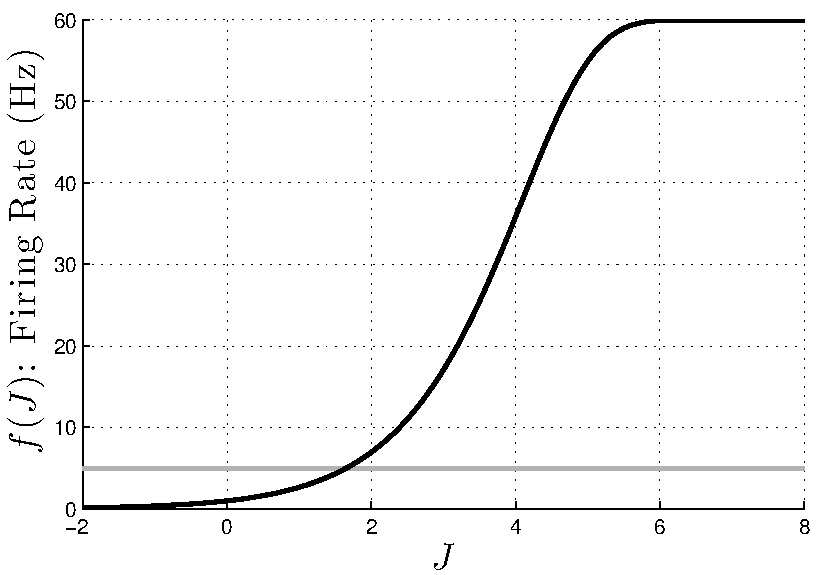
\includegraphics[width=3in]{../figs/fr_vs_J}
\caption{Expected firing vs. input to the neuron.  Given our model, Eq. \ref{eqn:glm:definition}, the relationship between firing rate and the magnitude of the input to a neuron is highly nonlinear.  Note that firing rate saturates at $1/\Delta$, because of our Bernoulli assumption.}
\label{fig:egfluor}
\end{figure}

Second, because the algorithms we develop below assume Markovian dynamics, we model the spike history terms as: 

\begin{equation} \label{eqn:h:definition} h_j(t) = (1- \Delta/\tau_h) h_j(t- \Delta) +n_j(t) + \sigma_h \sqrt{\Delta} \epsilon^h_j(t), \end{equation} 
	
where $\tau_h$ is the decay time constant for spike history terms, $\sigma_h$ is a standard deviation parameter, $\sqrt{\Delta}$ ensures that the statistics of this Markov process have a proper Ornstein-Uhlenbeck limit as $\Delta \to 0$, and throughout this paper, $\epsilon$ denotes an independent standard normal random variable. Note that this model generalizes (via a simple augmentation of the state variable $h_j(t)$) to allow each neuron to have several spike history terms, each with a unique time constant, which when weighted and summed allow us to model a wide variety of possible post-synaptic effects, including bursting, facilitating, and depressing synapses; see \cite{Vogelstein2009} for further details. In this paper, for simplicity, we assume that $\tau_h$ and $\sigma_h$ are known synaptic parameters, and therefore our model spiking parameters $\bth^n$ are given by $\{\bth^n_i\}_{i=1}^N$, where $\bth^n_i=\{\bw_i,k_i,b_i\}$, with $\bw_i=(\w_{i1},\ldots, \w_{iN})$.

The problem of estimating the connectivity parameters $\bw_i$ in this type of GLM, given a fully-observed ensemble of neural spike train $\{n_i(t)\}$, has recently received a great deal of attention; see the references above for a partial list. In the calcium fluorescent imaging setting, however, we do not directly observe spike trains; $\{n_i(t)\}$ must be considered a hidden variable here. Instead, each spike in a given neuron leads to a rapid increase in the intracellular calcium concentration, which then decays slowly due to various cellular buffering and extrusion mechanisms. We in turn make only noisy, indirect, and subsampled observations of this intracellular calcium concentration, via fluorescent imaging techniques \cite{ImagingManual}. To perform statistical inference in this setting, \cite{Vogelstein2009} proposed a simple conditional first-order hidden Markov model (HMM) for the intracellular calcium concentration $C_i(t)$ in cell $i$ at time $t$, along with the observed fluorescence $F_i(t)$: \begin{align} \label{eqn:ca:definition} C_i(t) &= C_i(t-\Delta) + (C_i^b-C_i(t-\Delta)) \Delta/\tau^c_i + A_i n_i(t)+\sigma^c_i \sqrt{\Delta} \epsilon^c_i(t), \\ F_i(t) &= \alpha_i S(C_i(t)) + \beta_i + \sqrt{\gamma_i S(C_i(t)) + \sigma^F_i} \epsilon^F_i(t). \label{eqn:F:definition} \end{align} This model can be interpreted as a simple driven autoregressive process: under nonspiking conditions, $C_i(t)$ fluctuates around the baseline level of $C_i^b$, driven by normally-distributed noise $\epsilon^c_i(t)$ with standard deviation $\sigma^c_i \sqrt{\Delta}$. Whenever the neuron fires a spike, $n_i(t)=1$, causing the calcium variable $C_i(t)$ to jump by a fixed amount $A_i$, and subsequently decay with time constant $\tau^c_i$. The fluorescence signal $F_i(t)$ corresponds to the count of photons collected at the detector per neuron per imaging frame. This photon count may be modeled with normal statistics, with the mean and variance given by generalized Hill functions, where $S(C)=C/(C+K_d)$ \cite{Yasuda2004}. Because the parameter $K_d$ effectively acts as a simple scale factor, and is a property of the fluorescent indicator, we assume throughout this work that it is known.

To summarize, Eqs. \ref{eqn:glm:definition} -- \ref{eqn:F:definition} define a coupled HMM: the underlying spike trains $n_i(t)$ and spike history terms $h_i(t)$ evolve in a Markovian manner, driving the intracellular calcium concentrations $C_i(t)$, which are themselves Markovian, but evolving at a slower timescale $\tau_i^c$. Finally, we observe only the fluorescence signals $\{F_i(t)\}$, which are related in a simple Markovian fashion to the calcium variables $C_i(t)$.


\subsection{Goal and general strategy}  \label{sec:methods:goal}

Our primary goal is to estimate the connectivity matrix, $\bw$, given the observed set of calcium fluorescence signals ${\bf F}$. We must also deal with a number of nuisance parameters: the spiking parameters $\{k_i, b_i\}$ and the calcium parameters $\{C^b_i, \tau^c_i, A_i, \sigma^c_i, \alpha_i, \beta_i, \gamma_i, \sigma^F_i\}$. We addressed the problem of estimating these latter parameters in earlier work \cite{Vogelstein2009}; thus our focus here will be on $\bw$. A Bayesian approach is natural here, since we have a good deal of prior information about neural connectivity; see \cite{Rigat06} for a related discussion. However, a fully-Bayesian approach, in which we numerically integrate over the very high-dimensional parameter $\theta = \{\bw, k_i, b_i, C^b_i, \tau^c_i, A_i, \sigma^c_i, \alpha_i, \beta_i, \gamma_i, \sigma^F_i\}$, is not particularly attractive here, from a computational point of view. Thus we take a compromise approach and compute \emph{maximum a posteriori} (MAP) estimates for the parameters via an expectation-maximization (EM) algorithm in which the sufficient statistics are computed by a hybrid blockwise Gibbs sampler and sequential Monte Carlo (SMC) method.

More specifically, we iterate the steps:
\begin{align*}
\textbf{E step} &\text{: Evaluate } Q(\bth^{(l+1)},\bth^{(l)}) =
E_{P[\bX | \bF; \bth^{(l+1)}]} \log P \left[ \bF, \bX | \bth^{(l)}
\right] = \int P[\bX | \bF; \bth^{(l+1)}] \log P[\bF, \bX | \bth^{(l)}]
d \bX \\ \textbf{M step} &\text{: Solve } \bth^{(l+1)} =
\argmax_{\bth} \left\{ Q(\bth,\bth^{(l)}) + \log P(\theta) \right\},
\end{align*}

where $\bX$ denotes the set of all hidden variables $\{ C_i(t), n_i(t), h_i(t) \}_{i \leq N, t \leq T}$ and $P(\theta)$ denotes a (possibly improper) prior on the parameter space $\theta$. According to standard EM theory \cite{DLR77,McLachlanKrishnan96}, each iteration of these two steps is guaranteed to increase the log-posterior $\log P(\bth^{(l+1)} | \bF)$, and will therefore lead to at least a locally maximum a posteriori estimator.

Now our major challenge is to evaluate the auxiliary function $Q(\bth^{(l+1)},\bth^{(l)})$ in the E-step. Because our model is a coupled HMM, as discussed in the previous section, $Q$ simplifies considerably \cite{RAB89}:

\begin{eqnarray}
  Q(\bth,\bth^{(l)}) &=& \sum_{it} P[C_i(t) | \bF; \bth] \times \log
P[F_i(t)|C_i(t); \alpha_i, \beta_i, \gamma_i, \sigma^F_i] \nonumber \\
&+& \sum_{it} P[C_i(t), C_i(t-\Delta), n_i(t) | \bF; \bth] \times \log
P[C_i(t)|C_i(t-\Delta), n_i(t); C^b_i, \tau^c_i, A_i, \sigma^c_i]
\nonumber \\ &+& \sum_{it} P[n_i(t), \bh(t) | \bF; \bth] \times \log
P[n_i(t)| \bh(t); b_i, k_i, \bw_i, S(t)],
\label{eqn:loglik:definition-expl}
\end{eqnarray}

where $\bh(t)=\{h_i(t)\}_{i=1}^N$. Thus we need only compute low-dimensional marginals of the full posterior distribution $P[\bX(t) | \bF; \bth]$; specifically, we need pairwise marginals, of the form $P[X_i(t), X_i(t-1) | \bF; \bth]$. The high dimensionality of the hidden variable $\bX$ necessitates the development of specialized blockwise Gibbs-SMC sampling methods, as we describe in sections \ref{sec:methods:indep} and \ref{sec:methods:joint} below. Once we have obtained these marginals, the M-step breaks up into a number of independent optimizations that may be computed in parallel and which are therefore relatively straightforward (section \ref{sec:methods:parameters HMM}); see section \ref{sec:methods:specific_implementation} for a pseudocode summary along with some specific implementation details.

\subsection{Initialization of ``internal'' parameters via sequential Monte Carlo methods} \label{sec:methods:indep}

We begin by constructing relatively cheap, approximate preliminary estimators for the nuisance parameters $\theta \backslash \bw$ (i.e., all of the parameters except the connectivity matrix $\bw$; that is, all of the parameters which are ``internal'' to neuron $i$). The idea is to initialize our estimate $\theta^{(0)}$ by assuming that each neuron is observed independently. Thus we want to compute $P[X_i(t), X_i(t-\Delta) | \bF_i; \bth_i]$, and solve the M-step for each individual parameter $\theta_i$, with the connection matrix $\bw$ held fixed. This single-neuron case is much simpler, and has been discussed at length in \cite{Vogelstein2009}; therefore, we only provide a brief overview here. The standard forward and backward recursions provide these posteriors \cite{ShumwayStoffer06}:

\begin{align}
  P[X_i(t) | F_i(0:t)] &\propto P[F_i(t)| X_i(t)] \int P[X_i(t)
| X_i(t-\Delta)] P[X_i(t-\Delta) | F_i(0:t-\Delta)] dX_i(t-\Delta)
\label{eqn:forward} \\ P[X_i(t), X_i(t-\Delta) | F_i] &= P[X_i(t) | F_i]
\frac{P[X_i(t) | X_i(t-\Delta)] P[X_i(t-\Delta) |
F_i(0:t-\Delta)]}{\int P[X_i(t) | X_i(t-\Delta)] P[X_i(t-\Delta) |
F_i(0:t-\Delta)] dX_i(t-\Delta)},
\label{eqn:backward}
\end{align}

where we have dropped the conditioning on the parameters $\theta$ for brevity's sake. Because these integrals cannot be analytically evaluated for our model, we approximate them using SMC (``marginal particle filtering'') methods \cite{DGA00,DFG01,GDW04}; see \cite{Vogelstein2009} for details on the proposal density and resampling methods used here. The output of these SMC techniques comprise an array of particle positions $\{X_i^{(l)}(t)\}$, where $l$ indexes the particle number, and a discrete approximation to the marginals $P[X_i(t), X_i(t-\Delta) | F_i]$,

\begin{equation}
  P[X_i(t), X_i(t-\Delta) | F_i] \approx \sum_{j,l}
  r_i^{(j,l)}(t,t-\Delta) \delta \left[ X_i(t) - X_i^{(l)}(t) \right]
  \times \delta \left[ X_i(t-\Delta) - X_i^{(j)}(t-\Delta) \right],
  \label{eq:particle-fb}
\end{equation}
where $r_i^{(j,l)}(t,t-\Delta)$ denotes the weight attached to the
particle pair with positions $\left( X_i^{(l)}(t), X_i^{(j)}(t-\Delta)
\right)$.

As discussed above, the sufficient statistics for estimating the
parameters for each neuron, $\bth_i$, are exactly these marginal
posteriors.  As shown in Eq. \ref{eqn:loglik:definition-expl}, the
M-step decouples into three independent subproblems.  The first term
depends on only $\{\alpha_i, \beta_i, \gamma_i, \sigma_i\}$; since
$\log P[F_i(t)|C_i(t); \theta_i]$ is quadratic (by our Gaussian
assumption on the fluorescent observation noise), we can estimate
these parameters by solving a weighted regression problem
(specifically, we use a coordinate-optimization approach: we solve a
quadratic problem for $\{\alpha_i, \beta_i\}$ while holding
$\{\gamma_i, \sigma_i\}$ fixed, then estimate $\{\gamma_i,\sigma_i\}$
by the usual residual error formulas while holding $\{\alpha_i,
\beta_i\}$ fixed).  Similarly, the second term requires us to optimize
over $\{\tau_i^c, A_i, C_i^b\}$ using a quadratic solver, and then we
use the residuals to estimate $\sigma_i^c$.  Note that all the
parameters mentioned so far are constrained to be non-negative, but
may be solved efficiently using standard quadratic program solvers.
Finally, the last term, assuming neurons are independent, may be
expanded:
\begin{equation} 
  E [\log P[n_i(t), \bh_i(t) | \bF; \bth]] = P[n_i(t), h_i(t) | F_i]
\log f (J_i(t)] + (1-P[n_i(t), h_i(t) | F_i]) \log [1- f(J_i(t))];
\label{eqn:bw}
\end{equation}
since $J_i(t)$ is a linear function of $(b_i,k_i,\bw_i)$, and the
right-hand side of (\ref{eqn:bw}) is concave in $J_i(t)$, we see that
the third term in \ref{eqn:loglik:definition-expl} is a sum of terms
which are concave in $(b_i,k_i,\bw_i)$, and may therefore be solved
efficiently using any convex optimization method, e.g.\ Newton-Raphson
or conjugate gradient ascent.

Our procedure therefore is to initialize the parameters for each
neuron using some default values that we have found to be effective in
practice, and then recursively (i) estimate the marginal posteriors (E
step), and (ii) maximize the parameters (M step), using the above
described approach.  We iterate these two steps until the change in
parameters does not exceed some minimum threshold.  We can then use
the marginal posteriors from the last iteration to seed the blockwise
Gibbs sampling procedure described below, to obtain a rough estimate
of $P[\bh(t) | \bF]$.

\subsection{Estimating joint posteriors over weakly coupled neurons}
\label{sec:methods:joint}

Now we turn to the key problem: computing $P(\bh(t),n_i(t) |
F,\theta)$, which encapsulates the sufficient statistics for
estimating the connectivity matrix $\bw$ (recall equation
(\ref{eqn:loglik:definition-expl})).  The SMC methods described in the
preceding section only provide the marginals over each neuron,
$P[X_i(t) | F_i; \bth_i]$; these methods may in principle be extended
to obtain the desired full posterior $P[\bX(t) | \bF; \bth]$, but
since the SMC algorithm is fundamentally a sequential importance
sampling method, these techniques scale poorly as the dimensionality
of the hidden state $\bX(t)$ increases \cite{BickelBengtsson08}.  Thus
we need a different approach.

One very simple idea is to use a Gibbs sampler: sample sequentially
from
\begin{align}
X_i(t) \sim P[X_i(t) | \bX_{\i}, X_i(0), \ldots, X_i(t-\Delta),
 X_i(t+\Delta), \ldots, X_i(T), \bF; \bth],
\end{align} 
looping in some order over all cells $i$ and all time bins $t$.
Unfortunately, this approach is likely to mix very poorly, due to the
strong temporal dependence between $X_i(t)$ and $X_i(t+\Delta)$.
Instead, we propose to use a blockwise Gibbs strategy, sampling each
spike train as a block:
\begin{align}
	X_i \sim P[X_i | \bX_{\i}, \bF; \bth];
\end{align} 
if we can draw these blockwise samples $X_i = \{X_i(t)\}$ efficiently
for a large subset of timebins $t$ simultaneously, then we would
expect the resulting Markov chain to mix much more quickly than the
naive element-wise Gibbs chain, since by assumption the hidden
variables $X_i,X_j$ are weakly dependent for different cells $i \neq
j$, and Gibbs is most efficient for weakly-dependent variables.

So, how can we efficiently sample from $P[X_i | \bX_{\i}, \bF; \bth]$?
One attractive approach is to try to repurpose the SMC methods
described above, which are quite effective for drawing approximate
samples from $P[X_i | \bX_{\i}, \bF_i; \bth]$ for one neuron $i$ at a
time.  Recall that sampling from an HMM is in principle easy by the
``propagate forward, sample backward'' method: we first compute the
forward probabilities $P[X_i(t) | \bX_{\i}(0:t), \bF(0:t); \bth]$
recursively for timesteps $0$ up to $T$, then sample backwards from
$P[X_i(t) | \bX_{\i}(0:T), \bF(0:T), X_i(t+\Delta); \bth]$.  This
approach is powerful because each sample requires just linear time to
compute (i.e., $O(T/\Delta)$ time, where $T/\Delta$ is the number of
desired time steps).  Unfortunately, in this case we can only compute
the forward probabilities approximately (with the SMC forward
recursion (\ref{eqn:forward})), and so therefore this attractive
forward-backward approach only provides approximate samples from
$P[X_i | \bX_{\i}, \bF; \bth]$, not the exact samples required to
establish the validity of the Gibbs method.

Of course, in principle we should be able to use the
Metropolis-Hastings (M-H) algorithm to correct these approximate
samples.  The problem is that the M-H acceptance ratio in this setting
involves a high-dimensional integral over the set of paths that the
particle filter might possibly trace out, and is therefore difficult
to compute directly.  \cite{Andrieu2007} discuss this problem at more
length, along with some proposed solutions.  However, a slightly
simpler approach was introduced by \cite{NBR03}.  Their idea is to
exploit the $O(T/\Delta)$ forward-backward sampling method by
embedding a discrete Markov chain within the continuous state space
$\mathcal{X}_t$; the state space of this discrete embedded chain is
sampled randomly according to some distribution $\rho_t$ with support
on $\mathcal{X}_t$.  It turns out that an appropriate acceptance
probability (defined in terms of the original state space model
transition and observation probabilities, along with the auxiliary
sampling distributions $\rho_t$) may be computed quite tractably,
guaranteeing that the samples produced by this algorithm form a Markov
chain with the desired equilibrium density.  See \cite{NBR03} for
details.

We can apply this embedded-chain method quite directly here to sample
from $P[X_i | \bX_{\i}, \bF; \bth]$.  The one remaining question is
how to choose the auxiliary densities $\rho_t$.  We would like to
choose these densities to be close to the desired marginal densities
$P[X_i(t) | \bX_{\i}, \bF; \bth]$, and conveniently, we have already
computed a good (discrete) approximation to these densities, using the
SMC methods described in the last section.  The algorithm described in
\cite{NBR03} requires that $\rho_t$ be continuous densities, so we
simply convolve our discrete SMC-based approximation (specifically,
the marginal of (\ref{eq:particle-fb})) with an appropriate normal
density to arrive at a very tractable mixture-of-Gaussians
representation for $\rho_t$.

Thus, to summarize, our procedure for sampling from the desired joint
state distributions $P(\bh(t),n_i(t) | F,\theta)$ has a
Metropolis-within-blockwise-Gibbs flavor, where the internal
Metropolis step is replaced by the $O(T/\Delta)$ embedded-chain method
introduced by \cite{NBR03}, and the auxiliary densities $\rho_t$
necessary for implementing the embedded-chain sampler are obtained
using the SMC methods from \cite{Vogelstein2009}.

\subsubsection{A cheaper high-SNR approximation of the joint posteriors}
\label{sec:cheaper-high-snr}

If the SNR in the calcium imaging is sufficiently high, then by
definition the observed fluorescence data $F_i$ will provide enough
information to exactly determine the underlying hidden variables
$X_i$.  Thus, in this case the joint posterior approximately
factorizes into a product of marginals for each neuron $i$:
\begin{equation} \label{eqn:indep_approx}
  P[{\bf X}|{\bf F};\theta] \approx \prod_{i=1}^N P[X_i|F_i; \bth].
\end{equation}
We can take advantage of this representation because we have already
estimated all the above marginals using the SMC methods described in
section \ref{sec:methods:indep}.  In particular, we can obtain the
sufficient statistics $P(\bh(t),n_i(t) | \bF,\theta)$ by forming a
product over the marginals $P(X_i(t) | \bF_i,\theta)$ obtained from
(\ref{eq:particle-fb}).  This approximation entails a very significant
gain in efficiency for two reasons: first, it obviates the need to
generate joint samples via the expensive blockwise-Gibbs approach
described above; and second, because we can very easily parallelize
the SMC step, inferring the marginals $P[X_i(t) | \bF_i; \bth_i]$ and
estimating parameters $\bth_i$ for each neuron on a separate
processor.  We will discuss the empirical accuracy of this
approximation in more depth in the Results section.


\subsection{Estimating the functional connectivity matrix} \label{sec:methods:parameters HMM}

Computing the M-step for the connectivity matrix, $\bw$, is an
optimization problem with on the order of $N^2$ variables.  By
construction, however, the auxiliary function
(\ref{eqn:loglik:definition-expl}) is concave in $\bw$, and decomposes
into $N$ terms which may be optimized independently using standard
ascent methods.  To improve our estimates, we will incorporate two
sources of strong \emph{a priori} information via our prior $P(\bw)$:
first, prior anatomical studies have established that connectivity in
many neuroanatomical substrates is ``sparse,'' i.e., most neurons form
synapses with only a fraction of their neighbors
\cite{Buhl94,Thompson88,Reyes98,Feldmeyer99,Gupta00,FeldmeyerSakmann00,PetersenSakmann00,Binzegger04,Song2005,Mishchenko2009b},
implying that many elements of the connectivity matrix $\bw$ are zero;
see also \cite{PAN04c,Rigat06,PILL07,Stevenson08} for further
discussion.  Second, ``Dale's law'' states that each of a neuron's
postsynaptic connections in adult cortex (and many other brain areas)
must all be of the same sign (either excitatory or inhibitory).  Both
of these priors are easy to incorporate in the M-step optimization, as
we discuss below.


\subsubsection{Imposing a sparse prior on the functional connectivity}

Enforcing sparseness for signal recovered with a series of linear
measurements via $L1$-regularizer is known to dramatically reduce the
amount of data necessary to accurately reconstruct the signal
\cite{Tibs96,TIP01,DE03,NG04,Candes2005,Mishchenko2009}.  We
incorporate a prior of the form $\log p(\bw) = const. - \lambda
\sum_{i,j} |\w_{ij}|$, and additionally enforce the constraints
$|\w_{ij}|<m$, for a suitable constant $m$ (since both excitatory and
inhibitory cortical connections are known to be bounded in size).
Since the penalty $\log p(\bw)$ is concave, and the constraints
$|\w_{ij}|<m$ are convex, we may still solve the resulting
optimization problem in the M-step using standard convex optimization
methods \cite{CONV04}.  In addition, the problem retains its separable
structure: the full optimization may be broken up into $N$ smaller
problems that may be solved independently.

\subsubsection{Imposing Dale's law on the functional connectivity}

Enforcing Dale's law requires us to solve a non-convex, non-separable
problem: we need to optimize the concave function $Q(\bth,\bth^{(l)})
+ \log P(\theta)$ under the non-convex, non-separable constraint that
all of the columns of the matrix $\bw$ are of a fixed sign (either
nonpositive or nonnegative).  It is difficult to solve this problem
exactly, but we have found that simple greedy methods are quite
efficient in finding good (possibly approximate) solutions.  We begin
with our original sparse solution, obtained as discussed in the
previous subsection without enforcing Dale's law.  Then we assign each
neuron as either excitatory or inhibitory, based on the weights we
have inferred in the previous step: i.e., neurons $i$ whose inferred
postsynaptic connections $w_{ij}$ are largely positive are tentatively
labeled excitatory, and neurons with largely inhibitory inferred
postsynapic connections are labeled inhibitory.  Neurons which are
highly ambiguous may be unassigned in the early iterations, to avoid
making mistakes from which it might be difficult to recover.  Given
the assignments $a_i$ ($a_i =1$ for putative excitatory cells, $-1$
for inhibitory, and $0$ for neurons which have not yet been assigned)
we solve the convex, separable problem
\begin{equation}
\argmax_{\substack{a_i \w_{ij} \geq 0 ~ \forall i,j}} Q(\bth,\bth^{(l)}) +
\log P(\theta),
\end{equation}
which may be handled using the standard convex methods discussed
above.  Given the new estimated connectivities $\bw$, we can re-assign
the labels $a_i$, or even flip some randomly to check for local
optima.  We have found this simple approach to be fairly effective in
practice.


\subsection{Specific implementation notes} \label{sec:methods:specific_implementation}

Pseudocode summarizing our approach is given in Algorithm
\ref{eqn:pseudocode}.  As discussed in section
\ref{sec:methods:indep}, the ``internal'' parameters $\theta
\backslash \bw$ may be initialized effectively using the methods
described in \cite{Vogelstein2009}; then the full parameter $\theta$
is estimated via EM, where we use the
embedded-chain-within-blockwise-Gibbs approach discussed in section
\ref{sec:methods:joint} (or the cheaper conditionally-independent
approximation described in section \ref{sec:cheaper-high-snr}) to
obtain the sufficient statistics in the E step and the separable
convex optimization methods discussed in section
\ref{sec:methods:parameters HMM} for the M step.

\begin{algorithm}
\caption{Pseudocode for estimating functional connectivity from
calcium imaging data using EM; $\eta^n$, $\eta^F$, $N_G$ are
user-defined convergence tolerance parameters.   XXX CAN WE INDENT
THE BELOW PROPERLY?  WOULD MAKE IT MORE LEGIBLE XXX}
\label{eqn:pseudocode}
\begin{algorithmic}
\While{$|{\bw}^{(l)}-{\bw}^{(l-1)}|>\eta^w$}
  \ForAll{$i=1\ldots N$}
    \While{$|{\bth_i}^{(l)}-{\bth_i}^{(l-1)}|> \eta^F$}
      \State Approximate $P[X_i(t)|F_i; \bth]$ using SMC (section
  \ref{sec:methods:indep})
      \State Perform the M-step for the ``internal'' parameters
  $\theta \backslash \bw$ (section \ref{sec:methods:indep}) 
    \EndWhile
  \EndFor
      \ForAll{$i=1\ldots N$}
      \State Approximate $P[n_i(t), \bh(t) |{\bf F}; \bth]$ using
  either the blockwise Gibbs method or the high-SNR
  conditionally-independent approximation (section \ref{sec:methods:joint})
    \EndFor
  \ForAll{$i=1\ldots N$}
  	\State Perform the M-step using separable convex optimization
  methods (section \ref{sec:methods:parameters HMM})  
  \EndFor
\EndWhile
\end{algorithmic}
\end{algorithm}

As emphasized above, the parallel nature of these EM steps is
essential for making these computations tractable.  We performed the
bulk of our analysis on a high-performance cluster of Intel Xeon L5430
based computers (2.66 GHz). For 10 minutes of simulated fluorescence
data, imaged at $30$ Hz, calculations typically took 10-20 minutes per
neuron using the conditionally-independent approximation, with time
split approximately equally between (i) estimating the internal
parameters $\theta \backslash \bw$, (ii) approximating the posteriors
using the independent SMC method, and (iii) estimating the functional
connectivity matrix, $\bw$.  The hybrid MCMC-Gibbs sampler was
substantially slower, up to an hour per neuron per Gibbs pass, with
the Gibbs sampler dominating the computation time (because the Gibbs process requires 5 Gibbs loops, each requiring about 5 MCMC forward-backward passes).





\section{Results}
\label{sec:results}
\subsection{Simulating neural activity in a neural population} \label{sec:results:simulations}

To test the described method for inferring functional connectivity from calcium imaging data, we simulated networks (according to our model, Eqs. \ref{eqn:glm:definition} -- \ref{eqn:F:definition}) of spontaneously firing randomly connected neurons.  Although simulations ran at $1$ msec time discretization, imaging rate was assumed to be much slower. Simulations lasted anywhere between 5 minutes and 1 hours (of simulated time).  Model parameters were chosen based on experimental data available in the literature
for cortical neural networks \cite{Braitenberg1998,Urquijo2000,Lefort2009,Sayer1990}.

More specifically, the network contained 80\% of excitatory and 20\% inhibitory neurons \cite{Braitenberg1998,Urquijo2000}, each respecting Dale's law. Neurons were randomly connected to each other with probability $0.1$ \cite{Braitenberg1998,Lefort2009}.  Synaptic weights for excitatory connections, as defined by EPSP peak amplitude, were randomly drawn from exponential distribution with the mean of $0.5 \mu V$ \cite{Lefort2009,Sayer1990}.
Inhibitory connections were also drawn from exponential distribution; their strengths chosen so as to balance excitatory and inhibitory currents in the network, and achieve an average firing rate of  $\approx 5 $ Hz \cite{Abeles01}. Practically, this meant that the mean strength of inhibitory connections was about 10 times larger than that of the excitatory connections.

Note that EPSP peak amplitudes cannot be used directly in Eq. \ref{eqn:glm:definition}. Really, $w_{ij}$ in Eq. \ref{eqn:glm:definition} is a dimensionless quantity representing the change in the spiking probability of neuron $i$ given neuron $j$ fired, while EPSP peak amplitude describes physiologically measured change in the membrane voltage of a neuron due to synaptic currents triggered by spike in neuron $j$. These two quantities, therefore, are dramatically different and we need to find a way to relate the two.

For that, we first point out that in order to trigger an immediate spike in a neuron that typically has its membrane voltage $V_b$ $\mu$V below the spiking threshold $n_E = V_b / V_E$ simultaneous EPSPs with the peak amplitude $V_E$ would be necessary.
Therefore, we propose that the change in the spiking probability of a neuron due to excitatory synaptic current $V_E$ can be approximately defined as
(so that $\delta P_E n_E \approx 1$)
\begin{equation}\label{eqn:convert:leadin-1}
\delta P_E = V_E/V_b.
\end{equation}
At the same time, according to Eq. \ref{eqn:glm:definition}, the same change in the spiking probability of a neuron $i$ following the spike of a neuron $j$ should be defined in GLM as
\begin{equation}\label{eqn:convert:leadin-2}
\delta P_E = \exp[-e^{b_i+w_{ij}}\tau_w]-\exp[-e^{b_i}\tau_w]
\end{equation}
Here $\tau_w$ is the typical EPSP time-scale, i.e. the time over which EPSP of one neuron, $j$, significantly affects the firing probability of the other neuron, $i$.

Equating Eq. \ref{eqn:convert:leadin-1} and Eq. \ref{eqn:convert:leadin-2}, we arrive at the proposition for our link function for physiologically measured EPSP peak amplitude, $V_E$, and GLM weight, $w_{ij}$:
\begin{equation}\label{eqn:convert}
\w_{ij}=\ln(-\ln(e^{-r_i\tau_w}-V_E/V_b)/r_i\tau_w).
\end{equation}
Here $r_i=\exp(b_i)$ is the base firing rate of neuron $i$. PSP shapes were modeled as an alpha function \cite{Koch99}, by differencing of two exponentials, corresponding to a sharp rise and relatively slow decay \cite{Sayer1990}.
%The time course of functional connectivity weights $\w_{ij}(t)$ was modeled as the difference of two exponentials, resulting in a rise time of $\tau_r=1$ msec and decay time of $\tau_{E_d}=10$ msec for excitatory and $\tau_{I_d}=20$ msec for inhibitory currents . In practice, we sampled time constants from uniform distributions with means as stated above and support of $\pm 25 \%$ of the means.
We neglected conduction delays, given that the time delay below $\sim 1$ msec expected in local cortical circuit was smaller than the time step of our computer simulation.  Each neuron also had an exponential refractory current \cite{Koch99}.

Parameters for the internal calcium dynamics and fluorescence observations were chosen according to our experience with several cells analyzed using algorithm of \cite{Vogelstein2009}, and conformed to other experimental observations \cite{ImagingManual,HelmchenSakmann96,BrenowitzRegehr07}. Each parameter was generated from a normal distribution with specified mean and variance at about 30\% of the mean, truncated at the lower bound at about 30\% of the mean value.  Table \ref{table:caparm} summarizes the details for each of the parameters in our model.

\begin{table}[h!b!p!]
\caption{Table of simulation parameters. $\mathcal{E}(\lambda)$ indicates an exponential distribution with mean $\lambda$, and $\mathcal{N}_p(\mu,\sigma^2)$ indicates a normal distribution with mean $\mu$ and variance $\sigma^2$, truncated at lower bound $p\mu$.}\label{table:caparm}

\begin{tabular}{ll}
\hline
Total neurons & 10-500 \\
Excitatory neurons & $80\%$ \\
Connections sparseness & $10\%$ \\
Baseline firing rate & 5 Hz\\
\hline
EPSP peak height 	& $\sim \mathcal{E}[0.5 \mu$V] \\
IPSP peak height 	& $\sim \mathcal{E}[2.3 \mu$V] \\
EPSP rise time 		& 1 msec \\
IPSP rise time 		& 1 msec \\
EPSP decay time 	& $\sim \mathcal{N}_{0.5}[10 $ msec$,(2.5 $ msec$)^2]$ \\
IPSP decay time 	& $\sim \mathcal{N}_{0.5}[20 $ msec$,(5 $ msec$)^2]$ \\
refractory time 	& $\sim \mathcal{N}_{0.5}[10 $ msec$,(2.5 $ msec$)^2]$ \\
\hline
Calcium std. $\sigma_c$ & $\sim \mathcal{N}_{0.4}[28\mu$M$,(10\mu$M$)^2]$ \\
Calcium jump after spike, $A_c$ &  $\sim \mathcal{N}_{0.4}[80\mu$M$,(20\mu$M$)^2]$\\
Calcium baseline, $C_b$ & $\sim \mathcal{N}_{0.4}[24\mu$M$,(8\mu$M$)^2]$ \\
Calcium decay time, $\tau_c$ & $\sim \mathcal{N}_{0.4}[200 $ msec$,(60 $ msec$)^2]$ \\
Mean photon budget $\alpha_c$ & $1$--$80$ Kph/neuron/frame \\
Dissociation constant, $K_d$ & $200 \mu$M \\
\hline
\end{tabular}
\end{table}


\subsection{Inferring functional connectivity from the simulated calcium imaging data} \label{sec:results:inference}

With neural population activity prepared as described in the previous section, we used our inference algorithms to reconstruct the functional connectivity matrix from simulated fluorescence data. Specifically, we estimated the connectivity matrix using both
the embedded-chain-within-blockwise-Gibbs approach as well as factorized approximation, Figure \ref{fig:scatters}.  We found that factorized approximation was able to provide reconstructions almost as accurate as the exact embedded-chain-within-blockwise-Gibbs approach --- $r^2=0.47$ versus $r^2=0.48$ --- when parameters corresponded to a realistic preparation, given $10$ minutes of simulation data, and a population of $N=25$ neurons.
We furthermore estimated the weights using GLM from the true spike trains, and the
true spike trains down-sampled to the frame rates  of calcium imaging,
$r^2=0.7$ and $r^2=0.57$ respectively.
thus, the quality of our estimates using the fluorescence traces was worse than those obtained from the the true down-sampled spike trainsm
although for SNR of fluorescence data the $r^2$ values for obtained reconstructions approached that of down-sampled true spike trains, Figure \ref{fig:recvar-SNR}.
Example of what we understand by high SNR (can be used for functional connectivity
inference) and low SNR (cannot be used for functional connectivity inference)
are shown in Figure \ref{fig:recvar-SNR} on two fluorescence traces from real
in-vivo data.

%Fluorescence data is generally acquired at low frame rate and, so, one of its main limitations is bad time-resolution of the observed spike trains. To determine the impact of this constraint on the connectivity reconstructions, and, thus, to determine how close calcium imaging may approach reconstructions from spike trains directly observed under comparable conditions, we conducted this experiment. We observed that at intermediate SNR reconstructions from calcium imaging closely resembled such obtained directly from spike trains, and at higher SNR reconstruction with the quality same with original spike trains was achieved, Figure \ref{fig:scatters} and \ref{fig:recvar-SNR}.


%\begin{align}
% \label{eqn:likelihoodGLMmoda}
% &E[\ln P[n_i(t)| \bh(t); b_i, k_i, \bw_i, S(t)]
% 	=\sum_t \left( n_i(t) \ln J_i(t) - (1-n_i(t)) \exp(J_i(t)) \Delta \right), \\
% \label{eqn:likelihoodGLMmodb}&J_i(t)=b_i+\sum\limits_j \sum\limits_{t'<t} \w_{ij}(t-t')n_{j}(t')=
% b_i+\sum\limits_j w_{ij} h_j(t).
% \end{align}

\comment{The sum in Eqs.\ref{eqn:likelihoodGLMmoda} and \ref{eqn:likelihoodGLMmodb} was over the sample of $\{n_i(t)\}$, produced with our spike sampling algorithm, discretized over the time-bins $t'$ with the width corresponding to the calcium imaging frame rate (i.e. 30 ms for 33 Hz and 15 ms for 66 Hz). In one of the two cases we considered, EPSP time-profiles were assumed to be ``known'' exponential, and the weights were estimated using reduced histories $h_{i}(t)=\sum_{t'<t} \exp(-(t-t')/\tau_h)n_{i}(t')$ with the time constant $\tau_h=10$ ms (i.e. second equation in Eq. \ref{eqn:likelihoodGLMmodb}). In the second case we considered, the time dependence of $\w_{ij}(t)$ was assumed to be unknown and the first equation in Eq. \ref{eqn:likelihoodGLMmodb}) was used to correlate $n_i(t)$ with $n_j(t')$ for $t'<t$ up to a given depth $m$.  In this latter case, since each next term in Eq. \ref{eqn:likelihoodGLMmodb}) was significantly smaller than the previous one, we found that the best results were obtained if we took $m=1$ (i.e. minimizing number of unknown variables given certain amount of data).
In either case, we described the connection weight between two neurons by a scalar quantity $w_{ij}^s=\text{sign}(\w_{ij})\max_{t} |\w_{ij}(t)|$, which thereafter was used to compare true and reconstructed connectivity weights in all examples below.}

\begin{figure}[h]
\centering
\begin{minipage}[c]{0.45\hsize}
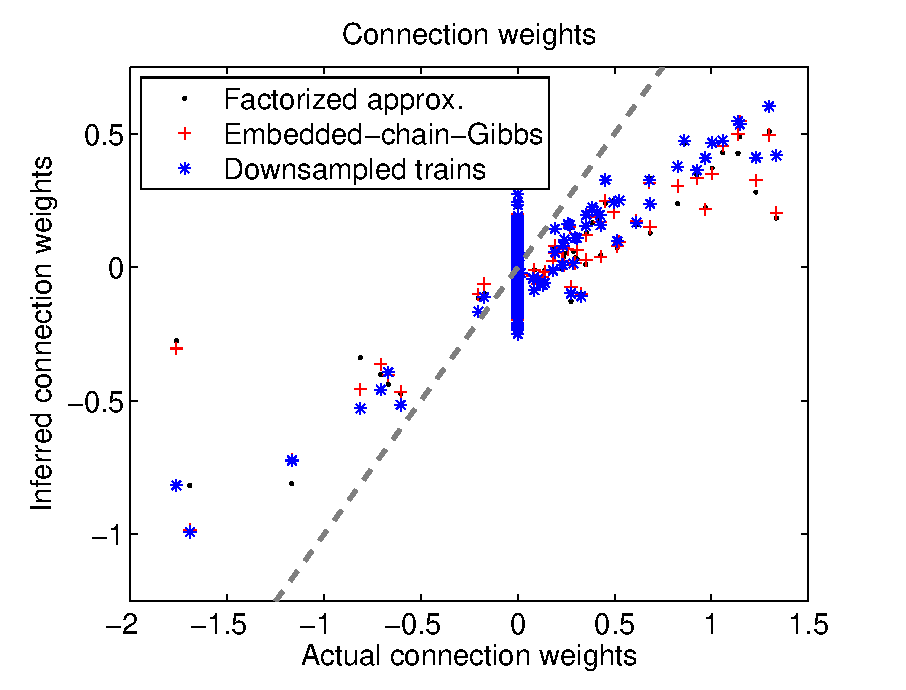
\includegraphics[width=\hsize]{../figs/FigureA3_scatter_three}
\end{minipage}
\begin{minipage}[c]{0.45\hsize}
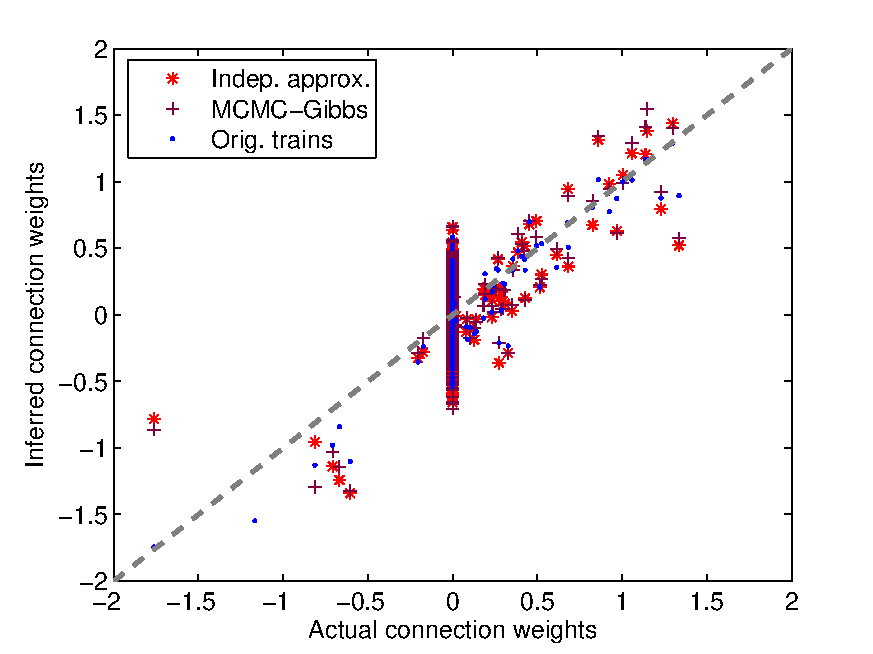
\includegraphics[width=\hsize]{../figs/FigureA3_scatter_three_corrected}
\end{minipage}
\caption{Functional connectivity matrix can be reconstructed from calcium imaging data.
Inferred connection weights are shown in a scatter plot versus real connection weights, with inference performed using factorized approximation, exact embedded-chain-within-blockwise-Gibbs approach, and true spike trains observed at the frame rate of the calcium imaging. Network of $N=25$ neurons was used, firing at $\approx 5$ Hz, and imaged for T=600 sec at intermediate SNR (photon budget 10Kph/neuron/frame, see below). $r^2=0.47$ for factorized approximation, $r^2=0.48$ for embedded-chain-within-blockwise-Gibbs, and $r^2=0.57$ for true down-sampled spike trains. Factorized approximation produced results almost as accurate as the exact embedded-chain-within-blockwise-Gibbs approach, and almost as accurate as the original spikes. Inferred connectivity weights were always scaled with respect to true connectivity due to time discretization bias (see main text).
This bias can be successfully calculated theoretically and removed from
the estimate of $\bw$.} \label{fig:scatters} \end{figure}

\subsection{Impact of coarse time discretization of calcium imaging data and scale bias in inferred connection weights}
Spike trains, necessary to evaluate functional connectivity matrix $\bw$, here were inferred with discretization into time-bins corresponding to the frame-rate of calcium imaging fluorescence data. In principle, one could use super-resolution feature of \cite{Vogelstein2009} to obtain spike trains with arbitrarily small time step $\Delta\rightarrow 0$. However, the problem in that case is that the spikes, inferred from fluorescence data, contain inaccuracy in their temporal position $\approx 1/$frame-rate,  due to the time-discretization of the underlying fluorescence trace.
Thus, when we super-resolve spikes using \cite{Vogelstein2009}, the spike pairs such that a spike of neuron $i$ closely follows a spike of neuron $j$ can be often confused with such where a spike of neuron $j$ closely follows a spike of neuron $i$.
It, therefore, becomes impossible to determine which neuron fired first, and which neuron
was pre-synaptic or post-synaptic in given pair of neurons $i$, $j$.
More specifically,
%because we rely on empirically counting close spike pairs in a set of spike trains to estimate the spike-triggered probabilities for spikes of different pairs of neurons, $i$ and $j$, which then allow estimating $w_{ij}$, above disordering of close spike pairs results in dramatic noise component in our estimate for the functional connectivity matrix by not allowing to effectively distinguish $w_{ij}$ and $w_{ji}$.
when using $\Delta \rightarrow 0$, we observed large errors in $\bw$,
$var[\bw] \propto \bw + \bw^T$ - because of inaccuracies in temporal position of spikes inferred from calcium imaging it became impossible to reliably distinguish which neuron causally preceded which other neuron, and only a-causal connectivity matrix $(\bw + \bw^T)/2$ could be determined.

To circumvent this problem, we (down-)sampled the time-axis in bins of size $\Delta=1/$frame-rate, and treated all spike pairs that occurred within the same time-bin as coincidental. This successfully counteracted the above problem and, additionally, allowed to perform calculations substantially faster by using larger $\Delta$. At the same time, this resulted in scale bias that all our inferred  connectivity matrices consistently exhibited, Figure \ref{fig:scatters}. This bias may be successfully understood and corrected from the following time-discretization argument.
Specifically, estimating the magnitude of the connection weight $w_{ij}$ is based on empirically evaluating the spike-triggered probability of neuron $i$ to fire, conditioned on neuron $j$. Most significant change in the spiking probability of neuron $i$, conditioned on neuron $j$, occurs within $\tau_w \approx 10-20$ msec from a spike of neuron $j$.
%To evaluate the magnitude of weight $w_{ij}$, therefore, we evaluate how many pairs of spikes, comprised of a spike of neuron $i$ following spike of neuron $j$ within $\approx \tau_w$, were empirically observed in a given spike train, and what spike-triggered probability this corresponds to.
When spike trains are down-sampled into large time-bins, e.g. $\Delta = 30$ msec, a significant fraction of close spike pairs appears coincident and not causal, as both spikes from neuron $i$ and neuron $j$ within $\approx \tau_w$ from each other are often assigned to the same time-bin.
As we discussed in the previous paragraphs, such close spike pairs typically introduce a great deal of noise in the estimate of $\bw$.
When $\Delta$ is large, however, most of such unreliable spike pairs would be considered coincidental and would not affect $\bw$ estimate. At the same time, all of such close pairs would be lost if we were to empirically evaluate the spike-triggered probabilities, which would have led us to believe in a lower than the actual  $w_{ij}$.


%
% Really, if the number of spikes of one neuron following that of another neuron within $\Delta$ was $n(2\rightarrow 1)$, while such in the reverse order was $n(1\rightarrow 2)$, difference $\delta n_{12} = n(2\rightarrow 1)-n(1\rightarrow 2)$ would correspond to the difference of functional connectivity weights $\delta w_{12}=w_{12}-w_{21}$. However, when such spike pairs had had their order confused with large probability $p\approx 1/2$, the number of spike pairs $n(2\rightarrow 1)$ actually observed would become $(1-p) n(2\rightarrow 1)+p n(1\rightarrow 2)$, and similarly for the reverse. Empirically observed difference $w_{12}-w_{21}$ thus would correspondingly drop to $\delta w'_{12}= (1-2p)\delta w_{12}$, while the variance would remain the same.
% We observed that the amount of data necessary to overcome this noise due to disordering of closely positioned spike-pairs appeared to be well over $\approx 10$ min of data used for the most of the calculations shown in this section below. Such high-time-resolution samples of spike trains also were substantially more computationally expensive to obtain and work with. For these reasons, we did not pursue this line of research further, although it may be of interest in the future.

To estimate the magnitude of this time-discretization bias quantitatively, we consider a significantly simplified case of two neurons coupled with a small weight $w_{12}$, and firing with baseline firing rate of $r=f(b)=\exp(b)$, $b \gg w_{12}$.
A sufficient statistics for estimating $w_{12}$ in this case is, e.g.:
\begin{equation}\label{eqn:scale:leadin-1}
\begin{array}{rl}
S =& E\left[\int\limits_{t'}^{t'+\mathcal{T}} \text{dt} n_1(t) | n_2(t')=\text{spike}, n_2(t)=\text{no spike}\ \forall t'<t<t'+\mathcal{T}\right] \\
\approx & r \mathcal{T} + f'(b) \int^{\mathcal{T}}  \text{dt} w_{12} \exp(-t/\tau_w) \\
\approx & r \mathcal{T} + f'(b) w_{12}\tau_w,
\end{array}
\end{equation}
where $\tau_w \ll \mathcal{T} \ll 1/r$, and
\begin{equation}\label{eqn:scale:leadin-1}
w_{12}=(S-r\mathcal{T})/f'(b)\tau_w.
\end{equation}
Now, if the spike trains were down-sampled into time-bins of size $\Delta$,
we estimate statistics $S$ with a discrete sum:
\begin{equation}\label{eqn:scale:leadin-2}
\begin{array}{rl}
S^{ds}=&E\left[\sum\limits_{t=t'+\Delta}^{t'+\Delta + \mathcal{T}} n^{ds}_1(t) | n^{ds}_2(t')=1, n^{ds}_2(t)=0\ \forall
t'<t<t'+\mathcal{T}\right]. \\
\approx& r \mathcal{T} + f'(b) \int\limits_0^\Delta \frac{\text{dt}'}{\Delta} \int\limits_{\Delta}^{\Delta + \mathcal{T}} \text{dt} w_{12}\exp(-(t-t')/\tau_w) \\
\approx & r \mathcal{T} +  f'(b)w_{12}\frac{1-\exp(-\Delta/\tau_w)}{\Delta/\tau_w^2}.
\end{array}
\end{equation}
$n^{ds}(t)$ here are down-sampled spikes, i.e. the spikes defined on a grid $t=0,\Delta,2\Delta,\ldots$.
In the second equality we took into account that the true position of the spike of the second neuron, $n^{ds}_2(t')$, may be uniformly distributed in first time-bin, here $[0,\Delta]$, and discrete sum over $t$ is from second time-bin $[\Delta,2\Delta]$ to $[\mathcal{T},\mathcal{T}+\Delta]$, i.e. over all spikes of the first neuron that occurred in any of the strictly subsequent time-bins up to $\mathcal{T} + \Delta$.
If we were to naively apply GLM Eq. \ref{eqn:scale:leadin-1} here using down-sampled estimate $S^{ds}$, we would have obtained
\begin{equation}\label{eqn:bias}
w_{12}^{ds}\approx \frac{1-\exp(-\Delta/\tau_w)}{\Delta/\tau_w} w_{12}.
\end{equation}
This is the scale bias that we observe.
In Figure \ref{fig:bias} we plot the scale bias from Eq. \ref{eqn:bias} versus that empirically deduced from our simulations for different values of $\Delta$. As can be seen in Figure \ref{fig:bias}, Eq. \ref{eqn:bias} describes observed scale bias very well.

\begin{figure}[h]
\centering
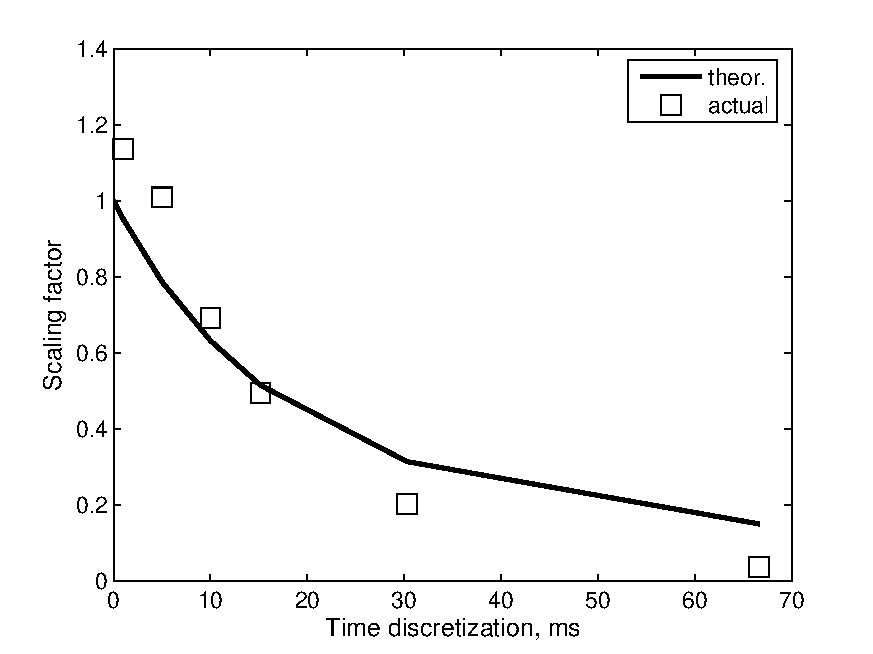
\includegraphics[width=3in]{../figs/FigureA4_scale_bias}
\caption{The low-frame rate of calcium imaging can explain the scale bias in inferred connectivity weights in Figure \ref{fig:scatters}.  Theoretically, scale bias may be evaluated by calculating what fraction of spikes from two neurons would occur within a single time-bin of width $\Delta$ (c.f. Eq. \ref{eqn:bias}).
Plotted such theoretically calculated scale bias (line) vs. that observed empirically from our simulations (box), from a simulation of $N=25$ neurons, $T=10$ min.
The error-bars correspond to 95\% confidence intervals for scale bias estimate.}
\label{fig:bias}
\end{figure}

\subsection{Impact of using priors on the inference}

\begin{figure}[h]
\centering
\begin{minipage}[c]{0.45\hsize}
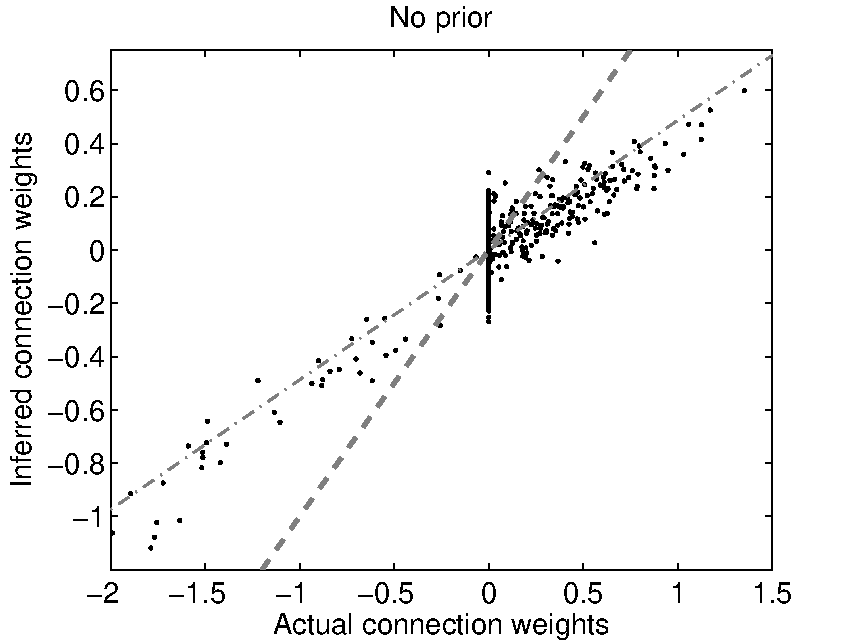
\includegraphics[width=\hsize]{../figs/FigureA10_regular_sol}
\end{minipage}
\begin{minipage}[c]{0.45\hsize}
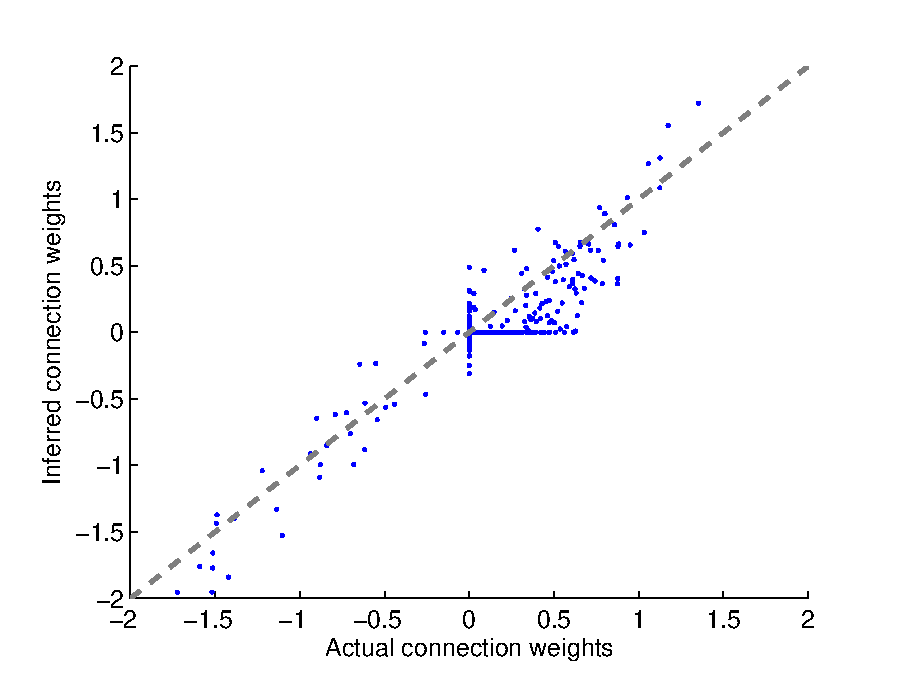
\includegraphics[width=\hsize]{../figs/FigureA10_sparse_sol}
\end{minipage}
\caption{
Incorporating simple priors on the distribution of connectivity weights, such as exponential sparseness prior, is essential to achieve much more accurate reconstructions from a smaller amount of calcium imaging data.
Shown here are the connection weights reconstructed using GLM (left panel) or sparse-prior GLM (right panel) are shown in a scatter plot for a network of $N=50$ neurons, firing at $\approx 5$ Hz, and imaged for $T=600$ sec. $r^2=0.64$ for simple GLM and $r^2=0.85$ for sparse-GLM.
Since original $\bw$ is sparse, noise in the estimates of $w_{ij}=0$ results in a vertical line at zero in the left panel.
Likewise, sparse prior results in many small $w_{ij}$ to be deduced as zeros, which produces the horizontal line at zero in the right panel.
}
\label{fig:sparse}
\end{figure}

\begin{figure}[h]
\centering
\begin{minipage}[c]{0.45\hsize}
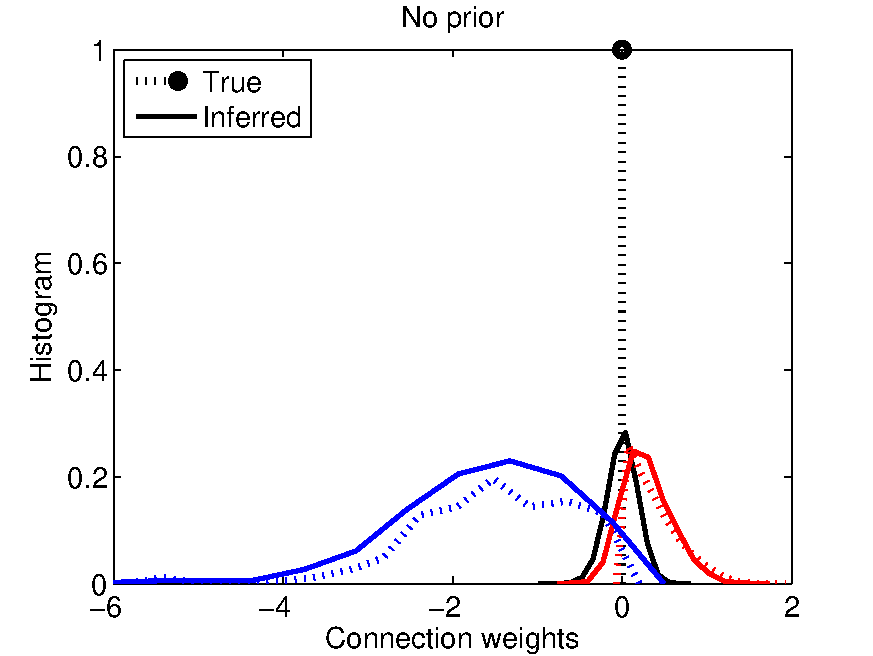
\includegraphics[width=\hsize]{../figs/FigureA3_hist_glm200}
\end{minipage}
\begin{minipage}[c]{0.45\hsize}
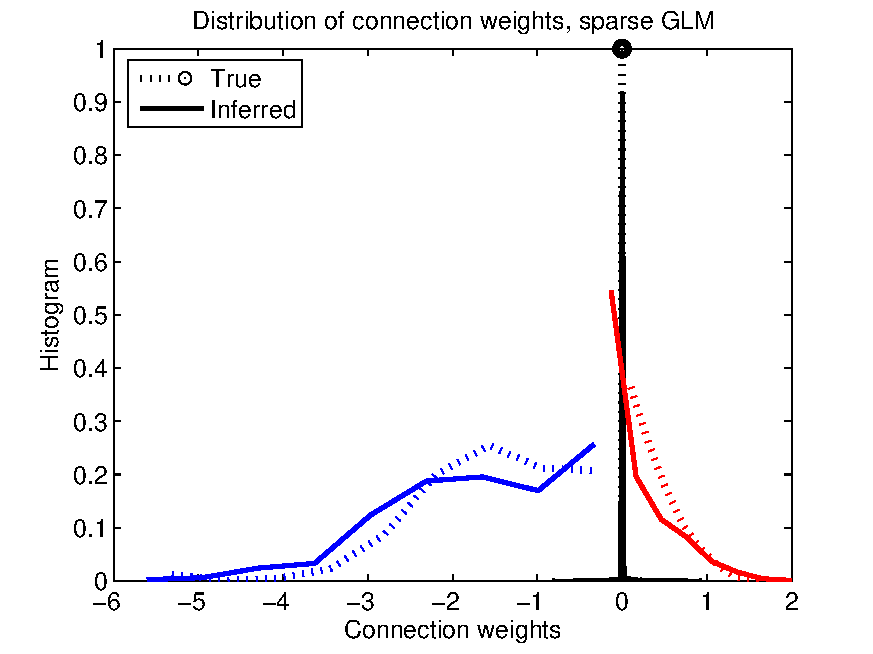
\includegraphics[width=\hsize]{../figs/FigureA3_hist_spa200}
\end{minipage}
\caption{
The distribution of inferred connection weights using GLM (left) and sparse GLM (right) vs. true distributions. When sparse exponential prior is enforced, dispersion in inferred connection weights is substantially reduced and, in particular, it becomes possible to reliably determine which neural pairs are connected, and which neurons are excitatory or inhibitory. Distributions are shown for a network of $N=200$ neurons, firing at $\approx 5$ Hz, and imaged for $T=600$ sec.}
\label{fig:distros}
\end{figure}


Taking into account simple prior information about the connectivity matrix results in dramatic improvement of the inferred connectivity matrix, Figure \ref{fig:sparse} and \ref{fig:distros}, allowing successful reconstruction from as little as 5 min of calcium imaging data, and for $T\approx 10$ min achieving the same level of accuracy otherwise requiring up to $T\approx 1$ hour of calcium imaging, Figure \ref{fig:recvar-NT}.
For example, in a network of $N=50$ neurons imaged for $T=10$ min, $r^2$ is increased from $r^2=0.64$ to $r^2=0.85$ when sparse prior was enforced.
Furthermore, $\bw$ estimates calculated with sparse prior allow reliable determination which neurons are connected, or which neurons are inhibitory or excitatory in nature, Figure \ref{fig:distros}.
At the same time, sparse prior introduces additional scale bias into connectivity estimates, which, therefore, effectively destroys information about the true scale of the connection weights.
Dale's prior, on the other hand, only leads to ~10\% in the correlation coefficient $r^2$ of the reconstructed connectivity matrix, and was not found significant. In case when sparse prior was initially enforced, enforcing Dale's prior typically resulted in no improvement to $\bw$ at all.


\subsection{Impact of different imaging frame rates, noise levels, and durations on the estimator accuracy}

\begin{figure}[h]
\centering
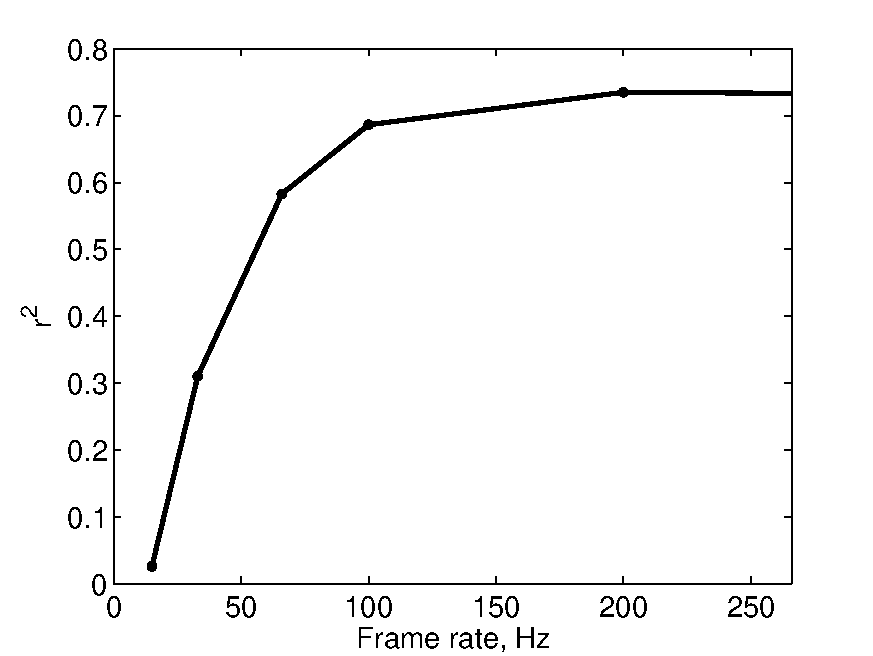
\includegraphics[width=3in]{../figs/FigureA5_recvar}
\caption{Accuracy of the inferred connectivity as function of the frame rate of calcium imaging. Connectivity matrix here was inferred from the original spike trains observed at corresponding frame rates, thus establishing the upper performance bound on the inference from calcium imaging data. A network of $N=25$ neurons, firing at $\approx 5$ Hz and imaged for $T=600$ sec was to generate this plot.}
\label{fig:recvar}
\end{figure}

\begin{figure}[h]
\centering
\begin{minipage}[c]{0.6\hsize}
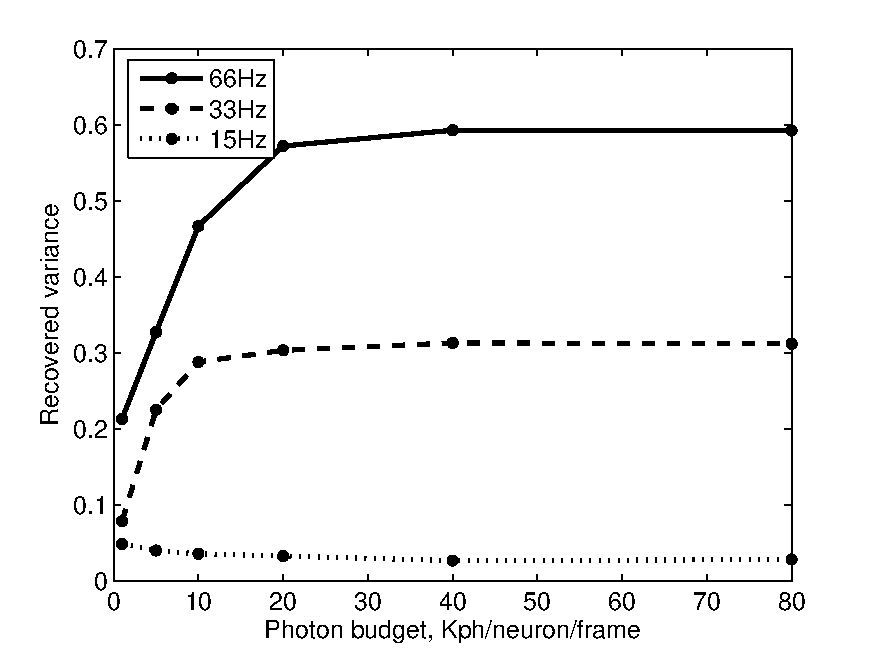
\includegraphics[width=\hsize]{../figs/FigureA6_recvar_SNR}
\end{minipage}
\begin{minipage}[c]{0.45\hsize}
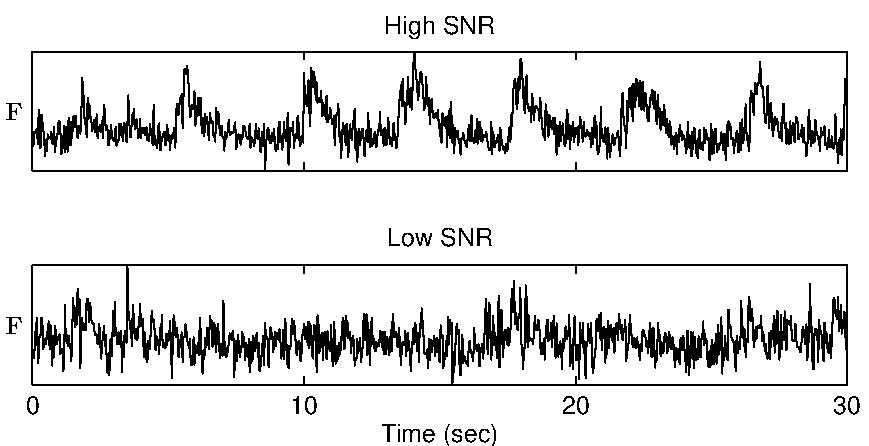
\includegraphics[width=\hsize]{../figs/example_traces}
\end{minipage}
\begin{minipage}[c]{0.45\hsize}
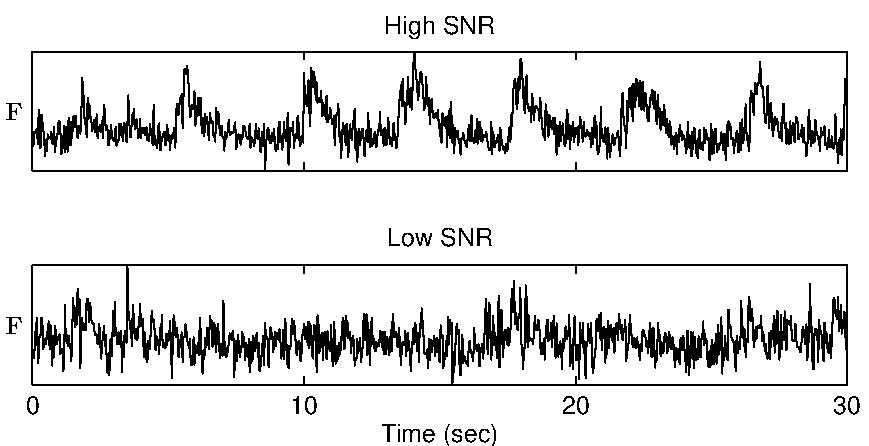
\includegraphics[width=\hsize]{../figs/example_traces}
\end{minipage}
\caption{Accuracy of inferred connectivity as function of the noise amount in the calcium imaging data, as quantified by photon budget, per neuron-frame, for frame rates of 15 Hz, 33 Hz and 66 Hz. Photon counts on the order of 10-20 Kph/frame/neuron are required to achieve the upper bound due by the frame rate. Connectivity matrix here was inferred from simulated fluorescence data using factorized approximation algorithm. Simulation conditions are the same as in Figure \ref{fig:recvar}.  Vertical black lines correspond to the two example traces in the lower panels, left to right respectively.}
\label{fig:recvar-SNR}
\end{figure}

\begin{figure}[h]
\centering
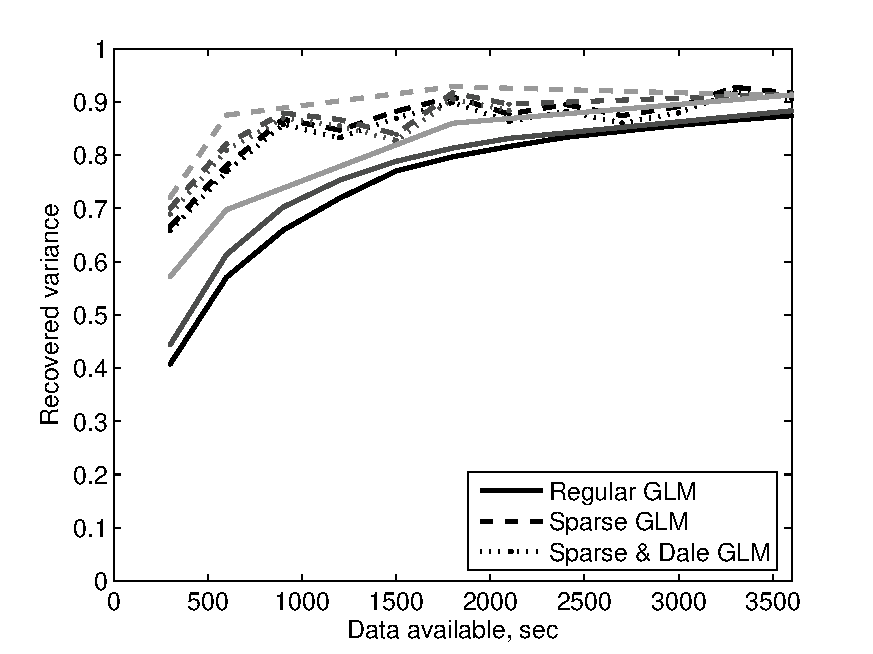
\includegraphics[width=3in]{../figs/FigureA7_recvar_NT}
\caption{Accuracy of inferred connectivity as function of the imaging time and neural population size. Incorporating simple priors such as exponential sparseness prior allows to boost dramatically the reconstruction's quality (dashed lines). In this latter case, $T=300$ sec is already sufficient to recover 70\% of the variance in the connection weights. Incorporating Dale's prior leads to only marginal improvement (dotted line). As shown in the methods, reconstruction accuracy does not depend on the neural population size $N$.
Here, neural population from $N=10$ to $N=200$ were simulated for different $T$, where
$N=200$ (gray) and $N=100$ (black) are shown. All networks were prepared in similar state by adjusting strength of inhibitory connections to achieve similar mean firing rate $\approx 5$ Hz, although actual firing rate could vary.
}
\label{fig:recvar-NT}
\end{figure}


What minimal conditions for the experimental setup should be met to allow successful reconstruction of the connectivity from calcium imaging data? In Figures \ref{fig:recvar} -- \ref{fig:recvar-NT} we address this question. Figure \ref{fig:recvar} shows the quality of the inferred connectivity matrix as function of the imaging frame rate - imaging frame rates 30-60 Hz are needed to achieve meaningful reconstruction results.
Frame rates $\approx 100$ Hz allow achieving the same level of the connectivity matrix reconstruction that is possible with the exact knowledge of the true spike trains.
Imaging frame 30-60 Hz are already possible in existing experimental setups, and imaging
at 100 Hz may be technologically possible in the future \cite{NguyenParker01,ReddySaggau05,Iyer06,SalomeBourdieu06,ReddySaggau08}

Figure \ref{fig:recvar-SNR} shows the quality of the inferred connectivity matrix as function of effective SNR and photon budget. Operationally, we define effective SNR as
\begin{equation}
eSNR=\frac{E[F_i(t)-F_i(t-1)|n_i(t)=1]}{E[{(F_i(t)-F_i(t-1))^2}/{2}|n_i(t)=0]^{1/2}},
\end{equation}

\noindent and photon budget as $\gamma^{-1}$. Photon budget corresponds to the number of photons collected from single neuron within a single frame, at the peak of fluorescence intensity. From our experience with the analysis of real cells \cite{Vogelstein2009}, the eSNR in real data was $\sim 3$ for in vivo data collected at 15  Hz and $\sim 9$  for in vitro data at the same frame rate. As can be seen from Figure \ref{fig:recvar-SNR}, the effective SNR necessary for accurate reconstructions was $\approx 5$. This eSNR corresponded to photon budgets of $\approx 10$ Kph/neuron/frame.
For lower eSNR, the amount of noise in calcium imaging data degraded inferred connectivity matrices significantly.

Finally, Figure \ref{fig:recvar-NT} shows the quality of the inferred connectivity matrix as function of the experiment duration. The minimal amount of data for a particular $r^2$ depended substantially on whether priors were enforced in M-step. In particular, for the M-step lacking a sparse prior, the calcium imaging duration necessary to achieve $r^2=0.5$ for the reconstructed connectivity matrix was $T\approx 10$ min, and $r^2=0.75$ was achieved at $T\approx 30$ min. When M-step enforced sparseness prior, $r^2>0.7$ was achieved already at $T\sim 5$ min. Furthermore, we observed that the accuracy of the reconstruction did not deteriorate with the size of the imaged neural population, whereas the same reconstruction quality was observed with the same amount of data for $N=50-200$ neurons.
This, at first unexpected, result is the direct consequence of the structure of the covariance matrix for $\bw$, as will be discussed below.
In all cases, good reconstructions were possible to obtain with only $T\sim 5$--$30$ min of calcium imaging data.


\subsection{Accuracy of the estimates and Fisher information matrix} \label{sec:methods:accuracy_Fisher}

Here we calculate theoretically the amount of spike trains data necessary to accurately estimate the functional connectivity matrix $\bw$. For clarity, we assume here that $\Delta \rightarrow 0$, and so $f(J)\approx e^J\Delta$, and that the spike trains are known perfectly, i.e. there is no corruption due to inference from low-SNR calcium imaging data.
As we shown above, for sufficient SNR this latter condition can be certainly achieved by calcium imaging data.
We also assume that the spikes only couple over a single time bin, i.e. $h_{ij}(t)\equiv n_j(t-\Delta)$.
Then, using GLM likelihood
\begin{equation}\label{eqn:fisher-glm}
\begin{array}{rl}
-\ln P[\bw | \bX] &\sim -\ln P[\bX | \bw] =
\sum\limits_{i,t} \left[ n_i(t) \ln f(J_i(t)) + (1-n_i(t)) (1-f(J_i(t))) \right], \\
J_i(t) &= b_i(t) + \sum\limits_j w_{ij} h_{ij}(t), \\
h_{ij}(t) &= n_j(t-\Delta),
\end{array}
\end{equation}
the Fisher information matrix for $P[\bw | \bX]$ is:
\begin{equation}\label{eqn:fisher-def}
\begin{array}{rl}
C^{-1}_{ij;i'j'}=\left[\frac{\partial (-\ln P[\bw | \bX])}{\partial \w_{ij}\partial \w_{i'j'}}\right]
=-&\delta_{ii'}\sum\limits_t\left[
n_i(t)n_{j}(t-\Delta)n_{j'}(t-\Delta)\left(-\frac{f'(J_i(t))^2}{f(J_i(t))^2} +
\frac{f''(J_i(t))}{f(J_i(t))}\right) - \right. \\
&\left.-(1-n_i(t))n_{j}(t-\Delta)n_{j'}(t-\Delta)f''(J_i(t))\right].
\end{array}
\end{equation}
where $f'$ and $f''$ correspond to the first and the second derivatives of our linking function (c.f Eq. \ref{eqn:glm:definition}), and $\delta_{ii'}$ is
the Kronecker's delta symbol, $\delta_{ii'}=1$ for $i=i'$, and $\delta_{ii'}=0$ otherwise.  Letting $f(J)=e^J\Delta$, the first term in the sum in Eq. \ref{eqn:fisher-def} cancels out, and the rest may be rewritten as:
\begin{equation}\label{eqn:fisher}
\begin{array}{rl}
C^{-1}_{ij;i'j'}
&=\delta_{ii'} T P[n_i(t)=0, n_j(t-\Delta)=1, n_{j'}(t-\Delta)=1]\times \\
&\times E[e^{J_i(t)}|n_i(t)=0, n_j(t-\Delta)=1, n_{j'}(t-\Delta)=1] \\
&= \delta_{ii'}T\left[(r \tau_w)\delta_{jj'}+O((r \tau_w)^2)\right]r.
\end{array}
\end{equation}
Here, $TP[n_i(t)=0, n_j(t-\Delta)=1, n_{j'}(t-\Delta)=1]$ describes the number of nonzero
terms in Eq. \ref{eqn:fisher-def}, corresponding to the condition that
$(1-n_i(t))n_{j}(t-\Delta)n_{j'}(t-\Delta)$ is only nonzero when
$n_i(t)=0, n_j(t-\Delta)=1, n_{j'}(t-\Delta)=1$.
$r=E[e^{J_i(t)}|n_i(t)=0, n_j(t-\Delta)=1, n_{j'}(t-\Delta)=1]$, then,
corresponds to the average value of $f''(J_i(t))$, conditional on such nonzero events.
$r\tau_w \ll 1$ is the probability for a neuron to spike over the time-interval  $\tau_w$.

The Fisher information matrix is block-diagonal, $C^{-1}_{ij;i'j'} \propto \delta_{ii'}$,
due to the structure of the log-likelihood $P[\bX | \bw]$, in particular, that it is represented as a sum over $i$ of independent terms, Eq. \ref{eqn:fisher-glm}.
But also from Eq. (\ref{eqn:fisher}) we observe that Fisher information matrix is predominantly diagonal, $C^{-1}_{ij;i'j'} \propto \delta_{ii'}\delta_{jj'}$, and thus the covariance matrix $C$can be computed trivially:
\begin{equation}
C = (rT)^{-1} (r \tau_w I + O((r \tau_w)^2))^{-1} =
(r^2 \tau_w T)^{-1} I + O((r \tau_w)^2)
\end{equation}

For successful determination of the functional connectivity matrix $\bw$, the variance $C$ should be made smaller than the typical scale $\langle \bw^2\rangle$, thus:
\begin{equation}
T \sim (\langle \bw^2 \rangle r^2  \tau_w)^{-1}.
\end{equation}
For typical values of $\bw^2\approx 0.1$, $r\approx 5$  Hz and $ \tau_w \approx 10$ msec,
with this order of magnitude estimate we obtain $T$ of the order of hundred seconds. This theoretical estimate of the necessary amount of fluorescent data is in good agreement with our simulations.

Finally, because $C^{-1}$ is diagonal, this scale of $C$ does not depend on the number of neurons in the imaged neural population, $N$. Thus, the variance of the estimate $\bw$ does not degrade with the size of the imaged population, $N$, for the same amount of data, $T$.

\subsection{Impact of strong correlations and deviations from generative model on the inference}

%Fig 7: non-robustness to strong correlations
%top panels: rasters
%bottom panels: corrected scatter plots
%
\begin{figure}[h]
\centering
\begin{minipage}[c]{0.45\hsize}
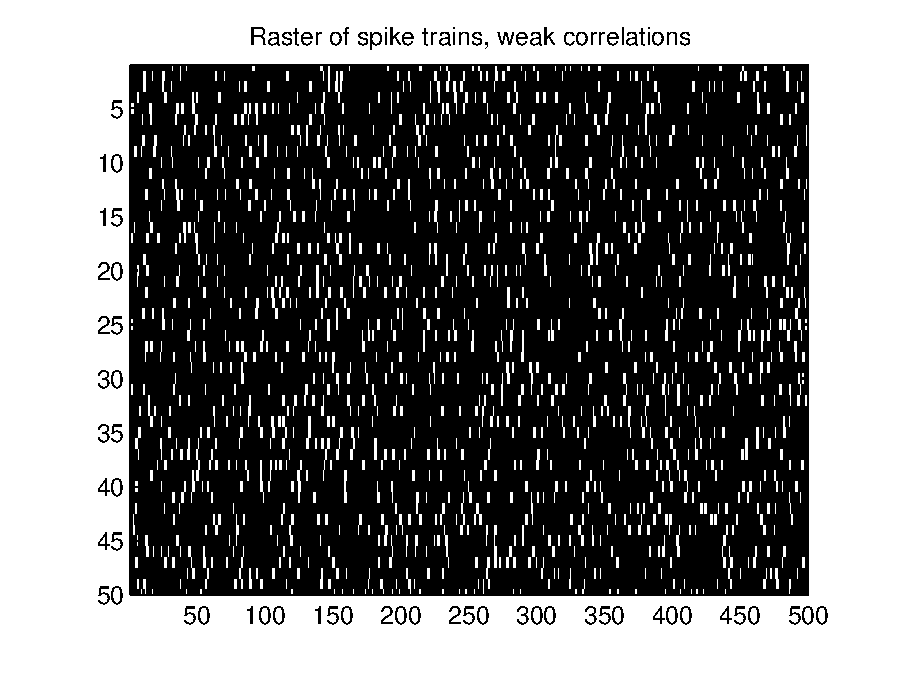
\includegraphics[width=\hsize]{../figs/Figure7b_raster_weak}
\end{minipage}
\begin{minipage}[c]{0.45\hsize}
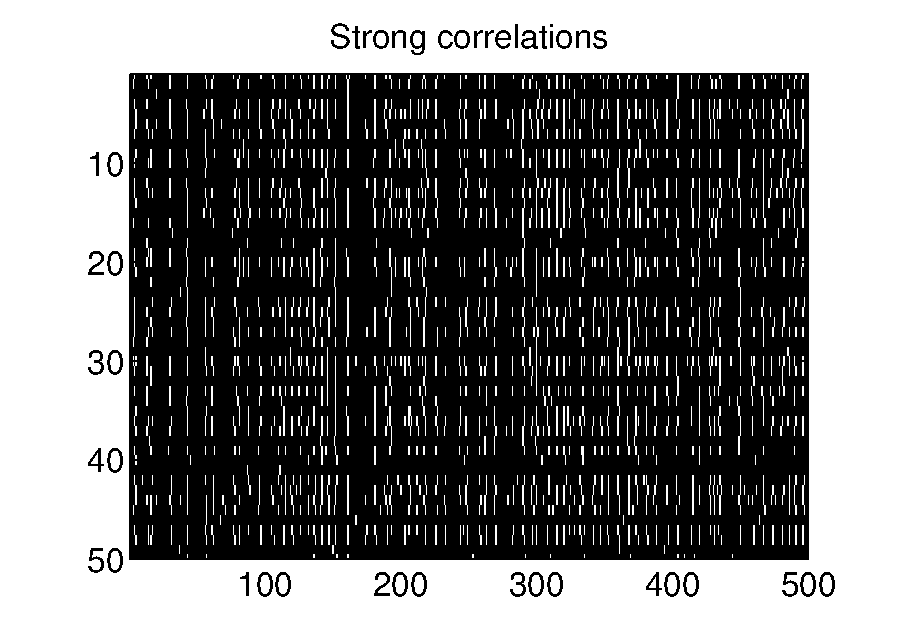
\includegraphics[width=\hsize]{../figs/Figure7a_raster_strong}
\end{minipage}
\begin{minipage}[c]{0.45\hsize}
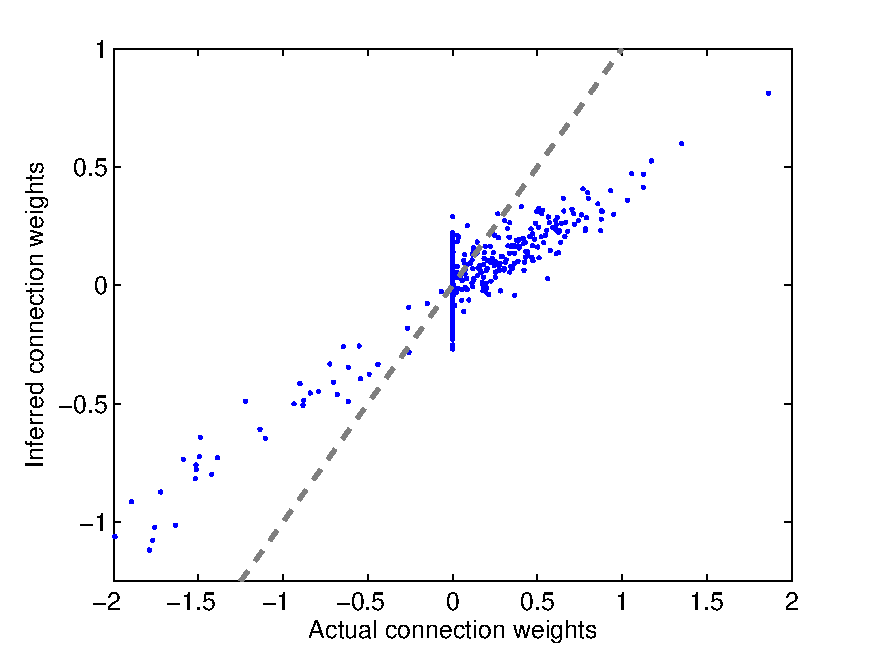
\includegraphics[width=\hsize]{../figs/FigureA8_weak_corr}
\end{minipage}
\begin{minipage}[c]{0.45\hsize}
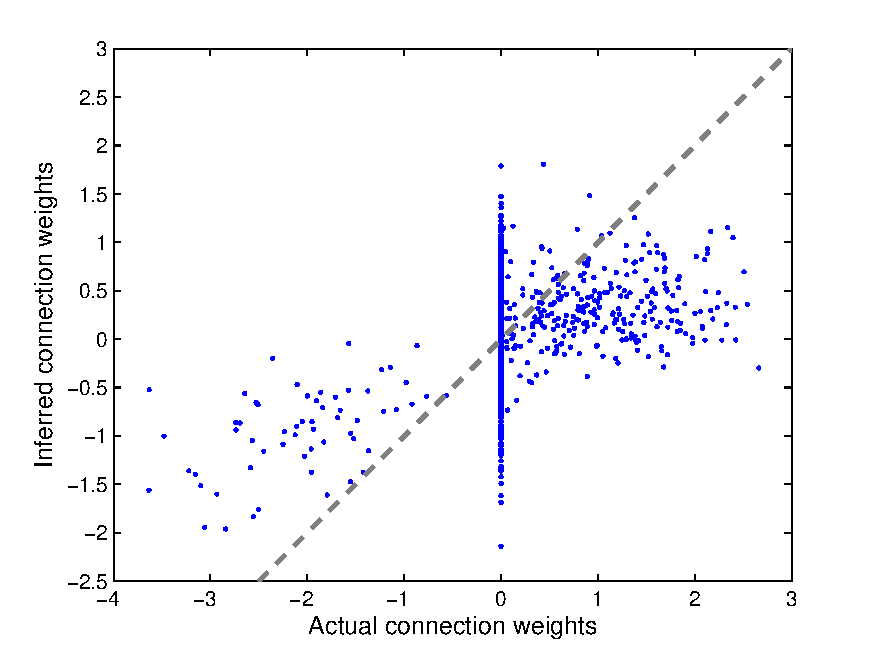
\includegraphics[width=\hsize]{../figs/FigureA8_strong_corr}
\end{minipage}
\caption{
Diverseness of observed neural activity patterns is required for
functional connectivity to give access to the actual ``anatomical'' structure
of the neural circuit. Here, 15 sec of simulated spike trains for a weakly coupled network (upper-left) and a network with strongly coupled component (upper-right) are shown.
In weakly coupled network spikes are sufficiently uncorrelated to give access to all different neural activity patterns needed to properly estimate true weights ${\bf w}_i$. In strongly coupled case, many instances of highly synchronous locked firings are evident, thus preventing observation of sufficiently rich ensemble of activity patterns.
Accordingly, GLM solution for the strongly coupled neural network (lower-right) does not
represent the true connectivity of the circuit, even for the weakly coupled component. This is contrary to the weakly-coupled network (lower-left) where true connectivity is successfully obtained.
Networks of $N=50$ neurons firing at $\approx 5$ Hz and imaged for $T=600$ sec were used to produce this figure.}
\label{fig:rasters}
\end{figure}

\begin{figure}[h]
\centering
\begin{minipage}[c]{0.45\hsize}
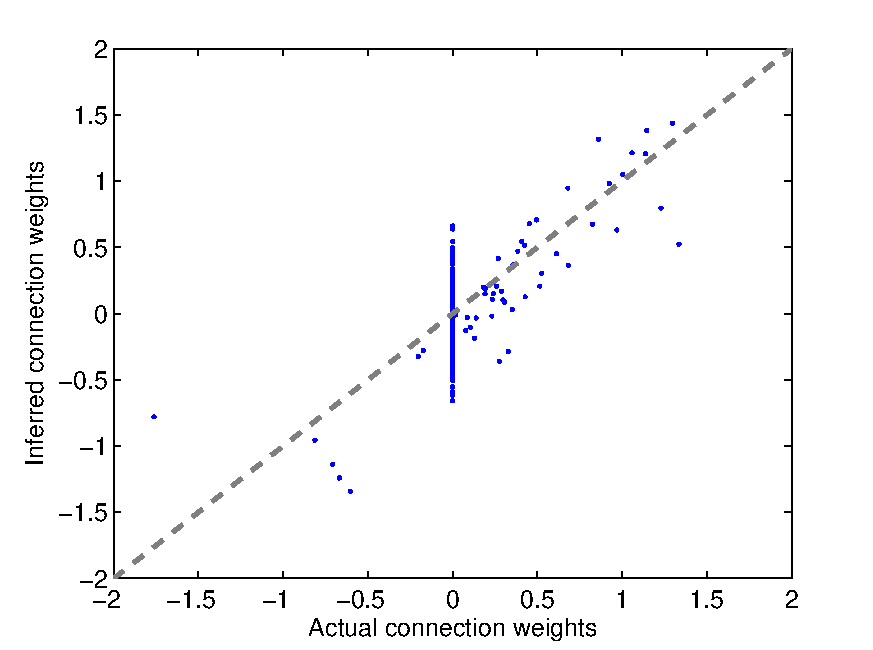
\includegraphics[width=\hsize]{../figs/FigureA9_all_same_sol}
\end{minipage}
\begin{minipage}[c]{0.45\hsize}
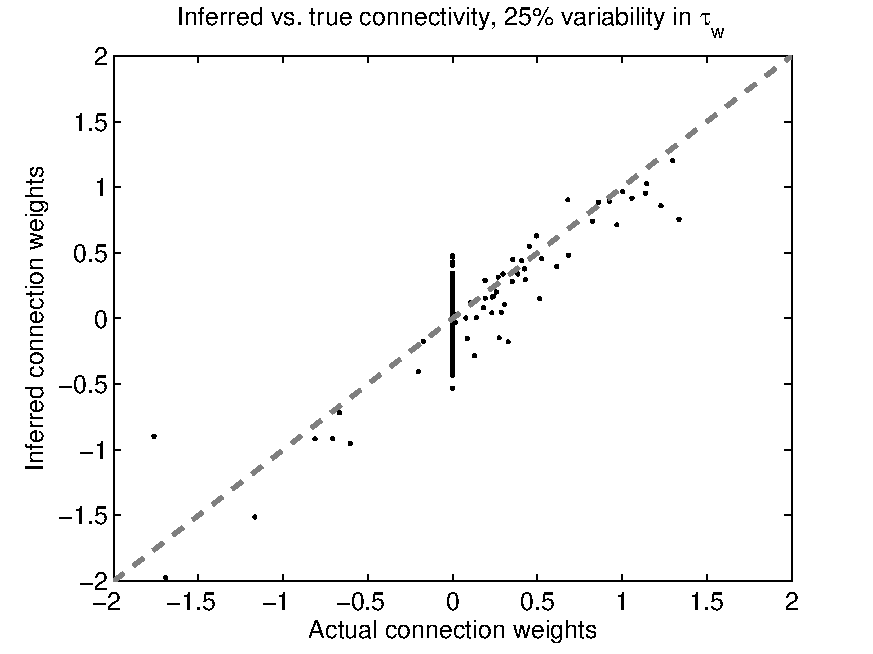
\includegraphics[width=\hsize]{../figs/FigureA9_variable_25}
\end{minipage}
\caption{Bayesian inference algorithm is robust to deviations of the
data from our generative model. One such deviation, that should be expected in real data, is variability in the EPSP time courses from neuron to neuron, and possibly synapse to synapse.
With up to 25\% variability allowed in EPSP time scales $\tau_w$ (right panel) our algorithm provided reconstructions of almost the same quality as when all $\tau_w$ were the same (left panel). Simulation conditions are the same as in Figure \ref{fig:recvar}.}
\label{fig:vartau}
\end{figure}


``Anatomical'' connectivity was recovered in our experiments despite potential problems noted in the literature [XXX], e.g. such as common input from correlated neurons. This is primarily due to the particular form of the activity in our neural networks, whereas firing of neurons occurred independently, thus, allowing GLM explore the full range of possible input configurations and disentangle common inputs.

Estimation of the functional connectivity is fundamentally routed in observing changes in the spike rate conditioned on the state of the other neurons. Intuitively, such estimation can be compared to observing changes in $f({\bf n}(t))\propto\exp(\sum_j \w_{ij}n_j(t))$ for different neural configurations ${\bf n}(t)$, i.e. estimating a vector ${\bf w}_i$ from a number of dot-products ${\bf w}_i\cdot {\bf n}(t)$. In order to properly estimate all components of ${\bf w}_i$ the set of available ${\bf n}(t)$ should be rich enough to span all $N$ dimensions of ${\bf w}_i$. In case of independent firing such condition is clearly satisfied.  Should this condition be violated, however, e.g. due to high correlation between spiking of few neurons, spike trains may not provide access to the true vector ${\bf w}_i$, and the connection weights inferred from such activity data may effectively ``aggregate'' true connection weights in arbitrary linear combinations.

We carried out a simulation of hypothetical ``strongly'' coupled  neural network, where in addition to weak sparse connectivity we introduced sparse random strong connectivity component. In a sense, we allowed a fraction of neurons to couple strongly to the other neurons, thus, making them ``command'' neurons ``driving'' the activity of the rest of the population. The strength of strong connectivity component was chosen to dynamically build up the actual firing rate from the baseline rate of $r=\exp(b)\approx 1$ Hz to $\approx 5$  Hz.
Such neural network showed patterns of activity very different from the weakly coupled networks inspected above, Figure \ref{fig:rasters}.  In particular, large number of highly correlated, synchronously locked firings of many neurons were evident in this network.  Likewise, our Bayesian algorithm was not able to identify the true connectivity matrix correctly, Figure \ref{fig:rasters}.

%Fig 8: robustness to variability in tau_h
%left: corrected scatter plot for (1) assuming same tau's, and (2) assuming they are all diff
%right: distributions of the weights, for truth and the above two approaches
%
%Fig 9: sparse glm improves fit (same format as Fig 8)
%




On the other hand, our inference algorithm showed significant robustness to deviations of the actual data from our generative model.
One important such deviation, which is likely to occur in the real experiments, is variation in the time-scales of EPSPs in different synapses. Up to now, all EPSP time-scales $\tau_w$ were assumed to be the same in our inference algorithm as well as in the simulations.
In Figure \ref{fig:vartau} we introduce additional variability in $\tau_w$ from one neuron to another.
Variability in $\tau_w$ results in added variance in the estimates of the connectivity weights $w_{ij}$ through $\tau_w$ dependence of the scaling factor Eq.(\ref{eqn:bias}).
Still, we found that such added variance was insignificant with $\tau_w$ varying for up to 25\% from neuron to neuron, Figure \ref{fig:vartau}.


%Fig -: real data
% \begin{figure}[h]
% \centering
% \begin{minipage}[c]{0.45\hsize}
% 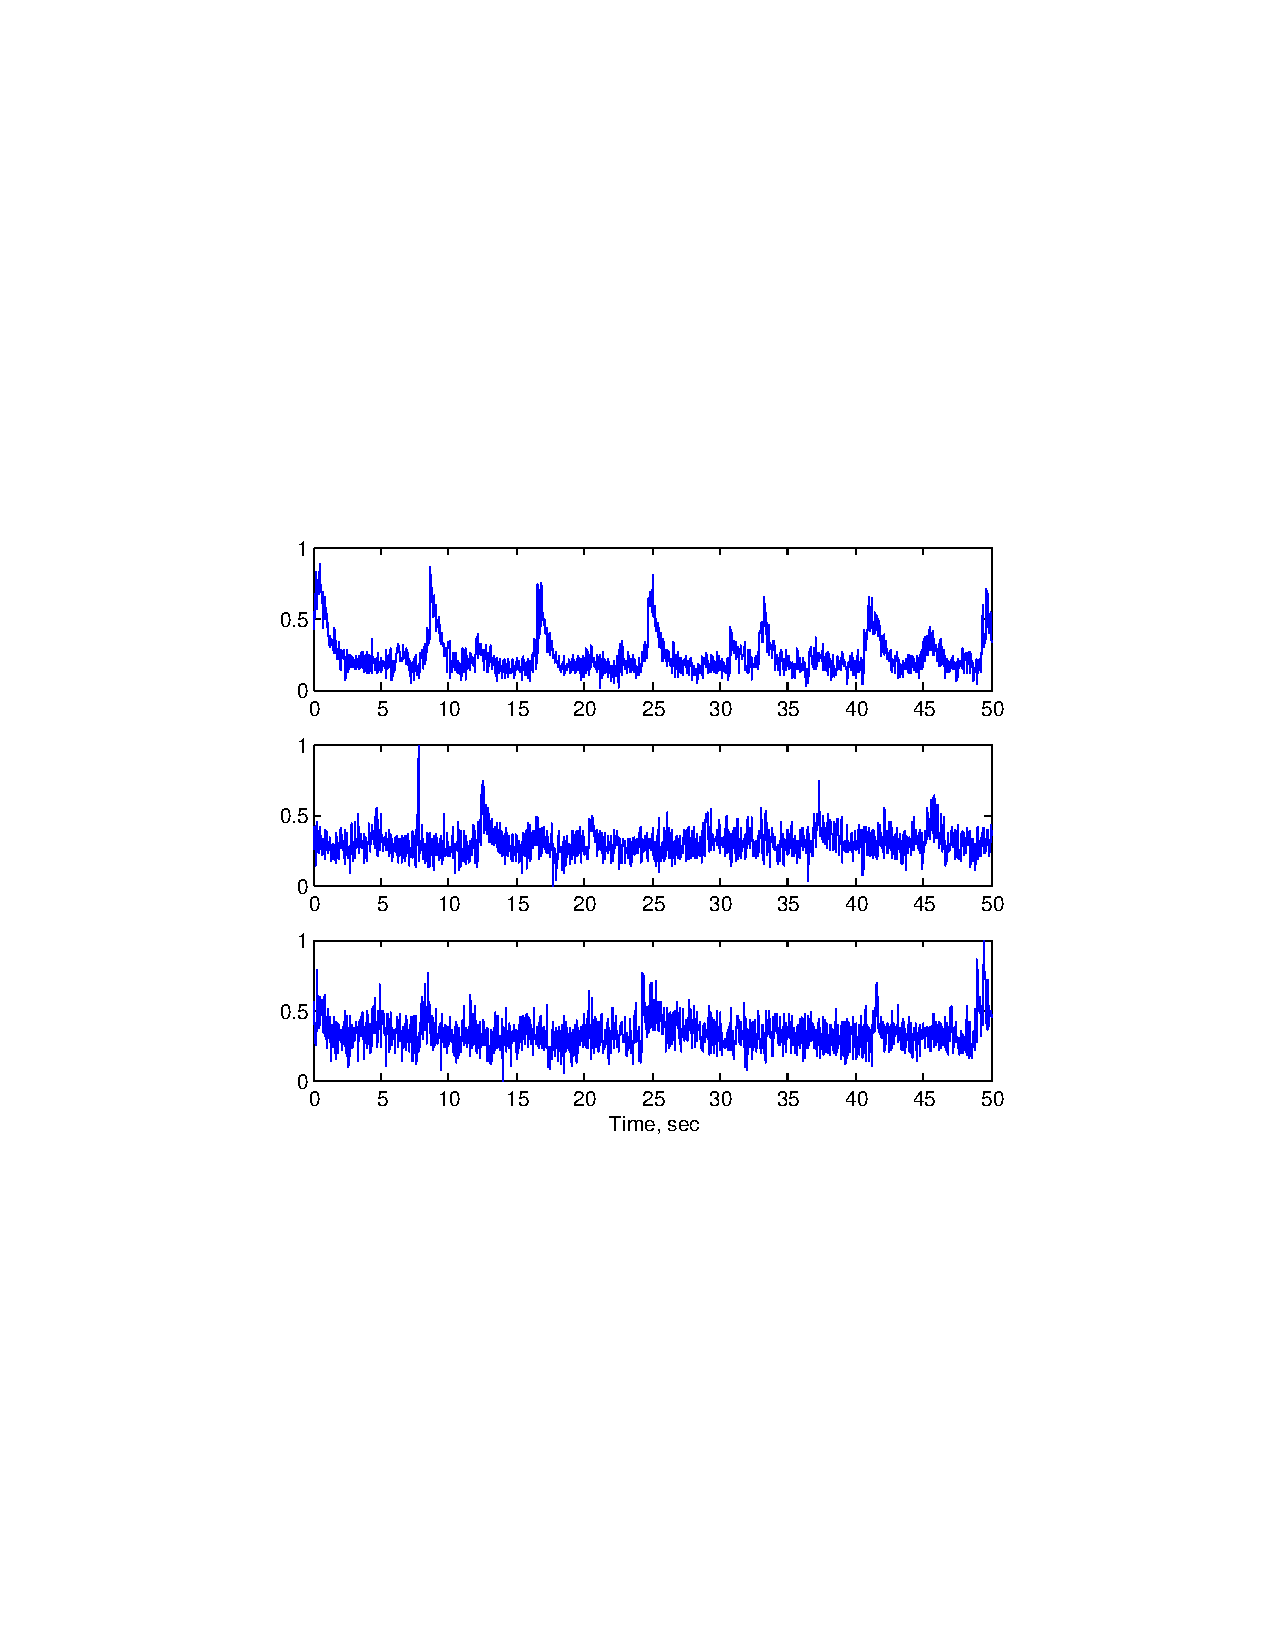
\includegraphics[width=\hsize]{../figs/FigureA11_real_traces}
% \end{minipage}
% \begin{minipage}[c]{0.45\hsize}
% 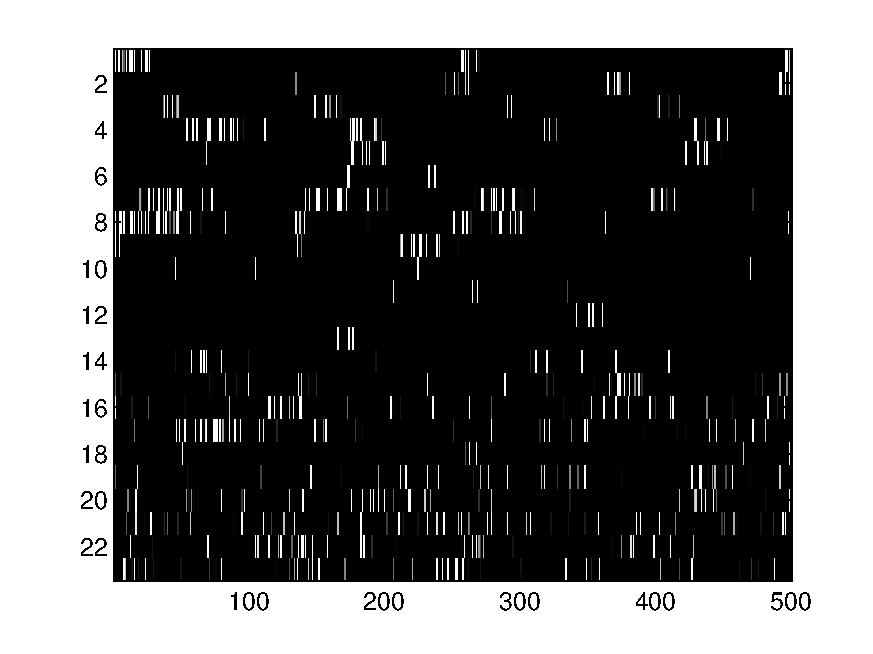
\includegraphics[width=\hsize]{../figs/FigureA11_real_raster}
% \end{minipage}
% \begin{minipage}[c]{0.3\hsize}
% 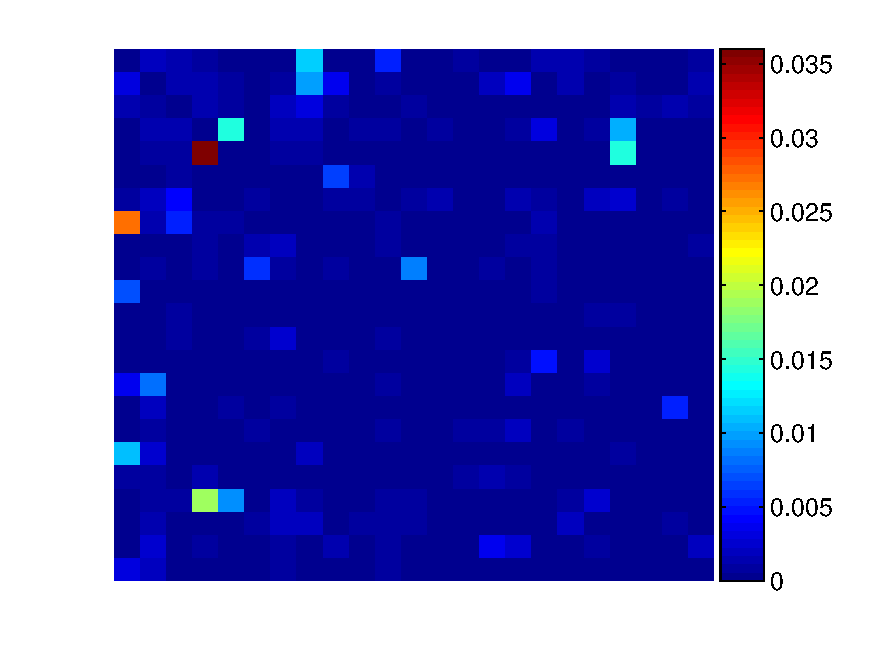
\includegraphics[width=\hsize]{../figs/FigureA11_real_Xcorr}
% \end{minipage}
% \begin{minipage}[c]{0.3\hsize}
% 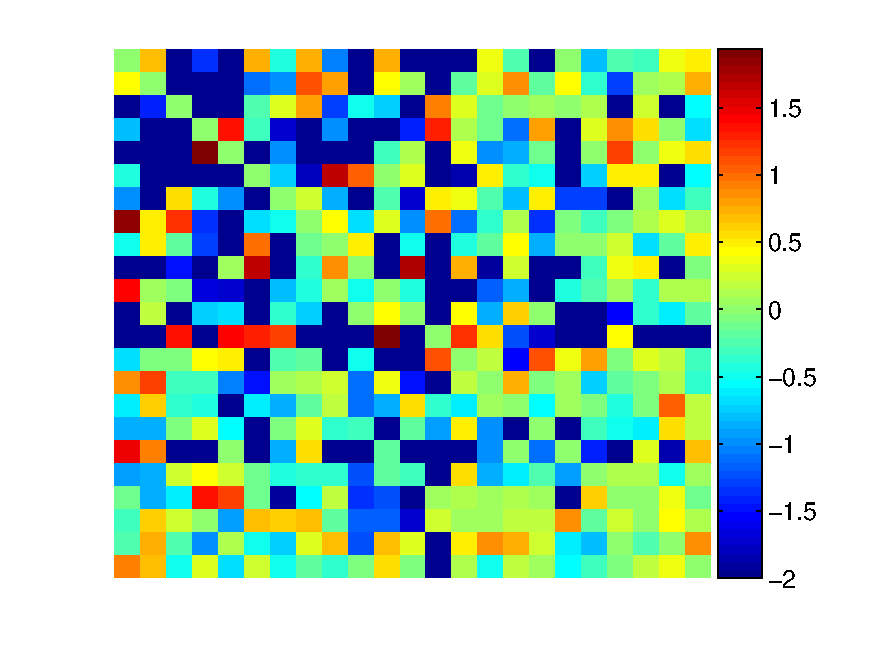
\includegraphics[width=\hsize]{../figs/FigureA11_real_glm}
% \end{minipage}
% \begin{minipage}[c]{0.3\hsize}
% 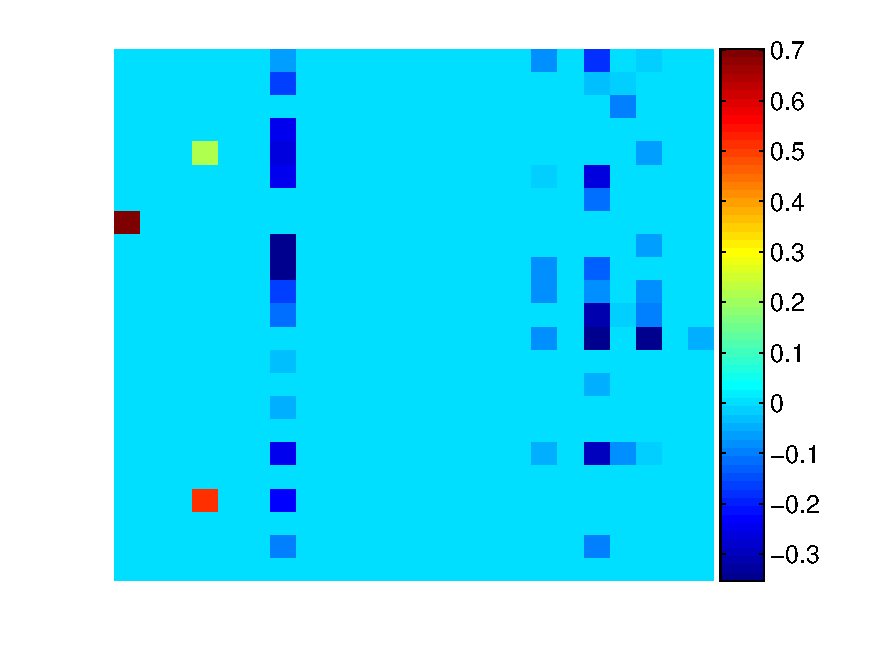
\includegraphics[width=\hsize]{../figs/FigureA11_real_sparse}
% \end{minipage}
% \caption{Functional connectivity matrix inferred from a sample of actual calcium imaging data for $N=72$ cells in [XXX], imaged for $T\approx 260$ sec at 15 Hz.
% $N=23$ neurons with spikes at sufficient SNR were selected, and functional connectivity reconstructed using factorized approximation algorithm. Firing cell of these cells was 0.1-1 Hz and 20-200 spikes were collected for each neuron.
% Upper-left panel shows example of actual fluorescence traces from selected cells, best to worst. Upper-right panel shows a raster of inferred spike trains for first 100 sec of imaging data. Lower panels show left-to-right the time-delayed cross-correlation matrix for selected neurons, simple GLM solution and sparse GLM solution, respectively. A consistent connectivity matrix is obtained here, with sparse solution having sparseness of $\approx 10 \%$, and all neurons automatically respecting Dale's law without explicitly enforcing it. Two clearly excitatory, and three clearly inhibitory neurons can be seen, with remaining neurons not showing significant couplings.}
% \label{fig:real}
% \end{figure}


%We applied our algorithm to a sample of the real calcium imaging data from [XXX], totaling about 5 minutes of imaging for a population of 72 cells in [XXX]. Out of these, about 23 cells had fluorescence traces indicative of spikes, while the other cells were either silent or did not shown SNR sufficient for analysis. These 23 cells were selected for futher processing. 20-200 spikes were found for each cell, corresponding to firing rates from 0.07 Hz to 0.8 Hz.
%We then identified functional connectivity matrix for this population. Sparse solution resulted in consistent connectivity matrix with sparseness of about 10\%, automatically respecting Dale's law, and clearly indicating two strongly connected excitatory neurons and few inihibitory neurons. Although this data lacked independent controls necessary to properly evaluate quality of our obtained reconstruction, it does demonstrate that our approach can be successfully applied under real-life condition to analyze functional connectivity of real populations of neurons.


\section{Discussion}
\label{sec:discussion}
Functional connectivity may fail to faithfully represent anatomical circuit structure if false correlations are present between different neurons, induced e.g. by common inputs, or if the dynamics of neural population is entirely concentrated on a low-dimensional subspace of the full configurational space ${\bf n}$. Note that these two statements are, in a sense, stating the same condition: if activity of different neurons is tightly correlated, their dynamics is concentrated on a low-dimensional plane and vice-versa - concentration of dynamics onto a low-dimensional plane will be perceived as correlation in activity of different neurons. In turn, low dimensionality of the neural dynamics may be caused by different factors, including common input, small subset of command neurons driving the circuit, or even emergent property of a network. Low dimensionality of neural dynamics results in that the inference problem becomes underdetermined, i.e. there may exist directions in ${\bf w}_i$ along which connectivity is not constrained by neural activity data (i.e. directions orthogonal to the subspace of all observed neural activity configurations), or is poorly constrained. This, naturally, leads to ${\bf w}_i$ being poorly defined along these directions. The necessary condition for good correspondence between functional connectivity weights ${\bf w}_i$ and anatomical connectivity, therefore, is {\em full-dimensionality} of the observed set of neural configurations. In case of spontaneously firing system of neurons this condition is satisfied by many neuron-firings occurring independently, thus, allowing to fully sample all possible directions in ${\bf w}_i$.  Still, spontaneously active preparation by itself may fail to display sufficient degree of independence between firing of neurons due to low-dimensionality of observed activity space, e.g. because of emergent properties of the circuit. In that case necessary variety of independent neural activity patterns may be enforced by randomly activating subsets of neurons via ChR2 or glutamate uncaging.

We also note that the correlations induced by secondary and so on synaptic transmissions (such as when neuron $A$ results in firing of neuron $B$, which in turn results in firing by neuron $C$), are all properly resolved in GLM-fitting process via the so called explaining-away process. In other words, because we do not just identify correlations between neural firings with the functional connectivity weights $\w_{ij}$, but instead statistically fit a model of neural interactions, if found weights between neurons $A$ and $B$, and $B$ and $C$ are sufficient to explain the correlation between $A$ and $C$, the weight connecting $A$ and $C$ will not appear in the model - the correlation between $A$ and $C$ was ``explained away'' by correlations between $A$ and $B$, and $B$ and $C$. By this, the multi-synaptic firing patterns do not confuse our estimation process.

ADD SOME RAVINGS ABOUT PROPER/IMPROPER FUNCTIONAL CONNECTIVITY.


% \begin{acknowledgments}
\section*{Acknowledgements}
Thank everyone for their help and support [Bows, Bows, Bows] !!!
% \end{acknowledgments}

\bibliography{mybib}
\bibliographystyle{amsplain}

\end{document}